%input macros (i.e. write your own macros file called MacroFile1.tex)
%\newcommand{\PdfPsText}[2]{
  \ifpdf
     #1
  \else
     #2
  \fi
}

\newcommand{\IncludeGraphicsH}[3]{
  \PdfPsText{\includegraphics[height=#2]{#1}}{\includegraphics[bb = #3, height=#2]{#1}}
}

\newcommand{\IncludeGraphicsW}[3]{
  \PdfPsText{\includegraphics[width=#2]{#1}}{\includegraphics[bb = #3, width=#2]{#1}}
}

\newcommand{\InsertFig}[3]{
  \begin{figure}[!htbp]
    \begin{center}
      \leavevmode
      #1
      \caption{#2}
      \label{#3}
    \end{center}
  \end{figure}
}


%%% Local Variables: 
%%% mode: latex
%%% TeX-master: "~/Documents/LaTeX/CUEDThesisPSnPDF/thesis"
%%% End: 


 \documentclass[oneside,12pt]{Classes/CUEDthesisPSnPDF}
\renewcommand\lstlistingname{Code}
\ifpdf
    \pdfinfo { /Title  (MSci Report)
               /Creator (Thomas William Rogers)
               /Producer (Thomas William Rogers)
               /Author (Thomas William Rogers thomas.rogers08@imperial.ac.uk@imperial.ac.uk)
               /CreationDate (D:20030101000000)  %format D:YYYYMMDDhhmmss
               /ModDate (D:20030815213532)
               /Subject (Density Matrix Quantum Monte Carlo)
               /Keywords (MSci, Thesis)}
    \pdfcatalog { /PageMode (/UseOutlines)
                  /OpenAction (fitbh)  }
\fi

\title{Density Matrix \\[1ex]
Quantum Monte Carlo}

\ifpdf
  \author{\href{mailto:thomas.rogers08@imperial.ac.uk}{Thomas William Rogers}}
  \collegeordept{\href{http://www3.imperial.ac.uk/physics}{Department of Physics}}
  \university{\href{http://www3.imperial.ac.uk}{Imperial College London}}
% insert below the file name that contains the crest in-place of 'UnivShield'
  \crest{
\includegraphics[width=40mm]{UnivShield}}
\else
  \author{Thomas William Rogers}
  \collegeordept{Department of Physics}
  \university{Imperial College London}
% insert below the file name that contains the crest in-place of 'UnivShield'
  \crest{
\includegraphics[bb = 0 0 292 336, width=30mm]{UnivShield}}
\fi
%
% insert below the file name that contains the crest in-place of 'UnivShield'
% \crest{\IncludeGraphicsW{UnivShield}{40mm}{14 14 73 81}}
%
\renewcommand{\submittedtext}{MSci Project Report}
\degree{{\small Supervisors: Prof. Matthew Foulkes \& Dr. James Spencer \\
Assessor: Dr. Alex Thom}}
\degreedate{}


% turn of those nasty overfull and underfull hboxes
\hbadness=10000
\hfuzz=50pt

% Put all the style files you want in the directory StyleFiles and usepackage like this:
%\usepackage{StyleFiles/watermark}

% Comment out the next line to get single spacing
\onehalfspacing

\begin{document}

%\language{english}

% A page with the abstract on including title and author etc may be
% required to be handed in separately. If this is not so, then comment
% the below 3 lines (between '\begin{abstractseparte}' and 
% 'end{abstractseparate}'), normally like a declaration ... needs some more
% work, mind as environment abstracts creates a new page!
% \begin{abstractseparate}
%   
% Thesis Abstract -----------------------------------------------------


%\begin{abstractslong}    %uncommenting this line, gives a different abstract heading
\begin{abstracts}        %this creates the heading for the abstract page
A new quantum Monte Carlo method based on stochastically sampling the thermal density matrix at finite temperatures has been developed. The method is an adaptation of the recently developed full configuration interaction quantum Monte Carlo\cite{Booth2009} (FCIQMC) method and it aims to overcome two of FCIQMCs main restrictions by allowing the calculation of any quantum mechanical observable at finite temperatures. During this report the density matrix quantum Monte Carlo (DMQMC) algorithm is formulated by observing an analogy with FCIQMC. It is then tested on the spin-$1/2$ antiferromagnetic Heisenberg model on a bipartite lattice.

The DMQMC method produces results that agree with the exact finite temperature FCI energy and exact ground-state staggered magnetisation for the $4\times4$ lattice. For the larger $6\times6$ lattice the standard DMQMC algorithm fails.  At this point an importance sampling method is introduced, yielding results comparable to accurate Green's function quantum Monte Carlo (GFQMC) estimates. The importance sampling method also enabled simulation of the $4\times4\times4$ lattice, producing results for the ground-state energy that matched those obtained by FCIQMC.

Finally an avenue into quantum information theory is explored and some key results for the entanglement between two qubits on a spin-$1/2$ antiferromagnetic Heisenberg ring are reproduced.  Additionally, both how the entanglement between qubits changes in a uniformly applied magnetic field and with increasing separation between the two qubits are investigated. 

\end{abstracts}
%\end{abstractlongs}


% ----------------------------------------------------------------------


%%% Local Variables: 
%%% mode: latex
%%% TeX-master: "../thesis"
%%% End: 

% \end{abstractseparate}




% Using the watermark package which is in StyleFiles/
% and to remove DRAFT COPY ONLY appearing on the top of all pages comment out below line
%\watermark{DRAFT COPY ONLY}


\maketitle

%set the number of sectioning levels that get number and appear in the contents
\setcounter{secnumdepth}{3}
\setcounter{tocdepth}{3}

\frontmatter % book mode only

%% Thesis Dedictation ---------------------------------------------------

\begin{dedication} %this creates the heading for the dedication page

I would like to dedicate this thesis to my loving parents ...

\end{dedication}

% ----------------------------------------------------------------------

%%% Local Variables: 
%%% mode: latex
%%% TeX-master: "../thesis"
%%% End: 

% Thesis Acknowledgements ------------------------------------------------


%\begin{acknowledgementslong} %uncommenting this line, gives a different acknowledgements heading
\begin{acknowledgements}      %this creates the heading for the acknowlegments

Thank you to Prof. Matthew Foulkes and Dr. James Spencer who thought of the original idea for this project and provided a great deal of help both in the physics and the computing that resulted in the achievement of these results. Many thanks also to my project-partner Nicholas Blunt, with whom the work in this project is equally shared. Finally, I am grateful for discussions on the application of DMQMC in quantum information theory with Dr. Terry Rudolph and of Tom Poole for proof-reading this report and offering some important changes.

This work made use of the Imperial College High Performance Computing facilities.


\end{acknowledgements}
%\end{acknowledgmentslong}

% ------------------------------------------------------------------------

%%% Local Variables: 
%%% mode: latex
%%% TeX-master: "../thesis"
%%% End: 


% Thesis Abstract -----------------------------------------------------


%\begin{abstractslong}    %uncommenting this line, gives a different abstract heading
\begin{abstracts}        %this creates the heading for the abstract page
A new quantum Monte Carlo method based on stochastically sampling the thermal density matrix at finite temperatures has been developed. The method is an adaptation of the recently developed full configuration interaction quantum Monte Carlo\cite{Booth2009} (FCIQMC) method and it aims to overcome two of FCIQMCs main restrictions by allowing the calculation of any quantum mechanical observable at finite temperatures. During this report the density matrix quantum Monte Carlo (DMQMC) algorithm is formulated by observing an analogy with FCIQMC. It is then tested on the spin-$1/2$ antiferromagnetic Heisenberg model on a bipartite lattice.

The DMQMC method produces results that agree with the exact finite temperature FCI energy and exact ground-state staggered magnetisation for the $4\times4$ lattice. For the larger $6\times6$ lattice the standard DMQMC algorithm fails.  At this point an importance sampling method is introduced, yielding results comparable to accurate Green's function quantum Monte Carlo (GFQMC) estimates. The importance sampling method also enabled simulation of the $4\times4\times4$ lattice, producing results for the ground-state energy that matched those obtained by FCIQMC.

Finally an avenue into quantum information theory is explored and some key results for the entanglement between two qubits on a spin-$1/2$ antiferromagnetic Heisenberg ring are reproduced.  Additionally, both how the entanglement between qubits changes in a uniformly applied magnetic field and with increasing separation between the two qubits are investigated. 

\end{abstracts}
%\end{abstractlongs}


% ----------------------------------------------------------------------


%%% Local Variables: 
%%% mode: latex
%%% TeX-master: "../thesis"
%%% End: 

\pagenumbering{roman}
\makeatletter
\@starttoc{toc}
\makeatother
\listoffigures
%{\RaggedRight
%\printnomenclature  %% Print the nomenclature
%}
%\addcontentsline{toc}{chapter}{Acronyms}

\mainmatter % book mode only
%%% Thesis Introduction --------------------------------------------------
\chapter{Introduction}
\ifpdf
    \graphicspath{{Introduction/IntroductionFigs/PNG/}{Introduction/IntroductionFigs/PDF/}{Introduction/IntroductionFigs/}}
\else
    \graphicspath{{Introduction/IntroductionFigs/EPS/}{Introduction/IntroductionFigs/}}
\fi
%%% ----------------------------------------------------------------------

%\nomenclature[z]{TISE}{Time-Independent  Schr\"{o}dinger equation}  
%The distribution and motion of electrons in a solid are described by the time-dependent Schr\"{o}dinger equation (TISE) . It is difficult to describe a macroscopic object accurately without considering the interactions between its constituent parts and in general such an object would consist of a number of constituent parts of the order of Avegadro's number. Solving the Schr\"{o}dinger equation for this many electrons proves extremely difficult. 

%A familiar approach is to replace the electron-electron interactions by a mean-field which allows the Schr\"{o}dinger equation to be separated into many single-body Schr\"{o}dinger equations.\cite{James1996} This mean field theory underpins much of current knowledge in solid-state physics and chemistry, but is found to fail for some ``strongly correlated''\footnote{A strongly correlated solid is one in which electrons experience strong Coulombic repulsion because of the spatial confinement of their orbitals \cite{Imada1998} . } solids, including rare earth metals and transition metal oxides.

\nomenclature[z]{QMC}{Quantum Monte Carlo} 
\nomenclature[z]{FCI}{Full configuration interaction} 
\nomenclature[z]{RNG}{Random number generator} 
The main aim of current electronic structure methods is to calculate the ground-state properties of many-electron systems. Conventional full-configuration interaction (FCI) calculations quickly become unfeasible because the size of the Hilbert space grows exponentially with the number of electrons. Such calculations based on iterative diagonalisation require the storage of at least as many double-precision numbers as twice the size of the Hilbert space \cite{Szabados2011}. 

Quantum Monte Carlo (QMC) methods can provide accurate simulations of many-electron systems via a stochastic sampling of the many-electron wave function. Such methods are favourable if the number of agents or ``walkers'' conducting the stochastic sampling is a small fraction of the size of the Hilbert space. 

Projector methods \cite{Kent1999} such as diffusion Monte Carlo (DMC) rely on the ground-state emerging from the imaginary-time Schr\"odinger equation in the limit of infinite imaginary-time (see Appx. A). However, because DMC does not enforce the constraint that a Fermionic wave function must be anti-symmetric, they suffer from convergence to the incorrect bosonic ground-state in an event known as the ``bosonic catastrophe''. In such cases the fixed-node approximation is applied \cite{Foulkes2001,BajdichMichalandMitas2009}, where \textit{a priori} knowledge of the wave-function is used to restrict the propagation of walkers so that they evolve towards an approximately antisymmetric solution.

%Quantum Monte Carlo (QMC) is a class of numerical algorithms which simulate quantum systems with the aim of solving the quantum many-body problem. The idea is to average a large number of ``computer experiments'', the result of which converges to the exact value of an observable. Surprisingly, with QMC methods it is possible to estimate expectation values for system observables without knowledge of the wave function for that system or enforcing a mean-field approximation. 
\nomenclature[z]{DMC}{Difussion Monte Carlo} 
Until recently QMC methods, such as DMC, could only provide numerically exact solutions for systems of many interacting bosons. The ``fermion sign problem'', described above, prevented an exact solution for systems of many interacting fermions. 

However, recently Booth \textit{et al.} \cite{Booth2009} introduced a new approach, known as full configuration-interaction QMC (FCIQMC), in which the antisymmetric property of the many-electron wave function is enforced by working in a discrete space of slater determinants (see Appx. A). The key is the improved efficiency of walker annihilation, which ensures convergence to the fermionic ground-state solution \cite{Spencer2012}.


\nomenclature[z]{FCIQMC}{Full configuration interaction quantum Monte Carlo}     
FCIQMC has two main restrictions. The first is that it proves difficult to calculate the expectation values of operators that do not commute with the Hamiltonian. The second being that it only allows for calculation of expectation values in the ground-state . This project introduces a method that is similar to FCIQMC, but attempts to overcome both of these restrictions. This is done by a stochastic sampling of the many-electron thermal density matrix as a function of inverse-temperature, rather than sampling the many-electron wave function as a function of imaginary-time. This in theory, allows for the calculation of the expectation values of any operator at finite temperatures.

\nomenclature[z]{DMQMC}{Density matrix quantum Monte Carlo} 
\nomenclature[z]{GFQMC}{Green's function quantum Monte Carlo} 
In Ch.~\ref{ch:chapter1} the density matrix quantum Monte Carlo (DMQMC) algorithm is developed and an optimised and highly parallel implementation is discussed. In Ch.~\ref{ch:chapter2} DMQMC is applied to the spin-$1/2$ antiferromagnetic Heisenberg model on two and three dimensional bipartite lattices. The results are compared against exact values from the full diagonalisation of the Hamiltonian, for small systems, and accurate FCIQMC or Green's function QMC (GFQMC) estimates for larger systems. Finally, in Ch.~\ref{ch:chapter3} a method of calculating a reduced density matrix for a subsystem of the Heisenberg lattice is developed and this leads into applications in quantum information theory.

Note that a system of units with $\hbar = k_B = 1$ is adopted for all equations in this report.



%%% Local Variables: 
%%% mode: latex
%%% TeX-master: "../thesis"
%%% End: 

\chapter{The DMQMC algorithm}
\label{ch:chapter1}
\ifpdf
    \graphicspath{{Chapter1/Chapter1Figs/PNG/}{Chapter1/Chapter1Figs/PDF/}{Chapter1/Chapter1Figs/}}
\else
    \graphicspath{{Chapter1/Chapter1Figs/EPS/}{Chapter1/Chapter1Figs/}}
\fi

In this chapter the DMQMC algorithm is formulated using an analogy between the imaginary-time Schr\"odinger equation and the evolution of the many-electron thermal density matrix as a function of inverse-temperature. Several features of FCIQMC are used in the construction of this algorithm in a way that maintains FCI-quality results. Finally, the main features of an optimised and highly parallel implementation of the DMQMC algorithm are discussed.

\section{The thermal density matrix}
\label{sec:DensityMatrix}

In quantum mechanics the density operator\cite{Isham} is any operator, $\rho$, that satisfies three properties:
\begin{enumerate}
\item It is Hermitian i.e. $\rho = \rho^{\dag}$
\item It is a positive, semi-definite operator, i.e. $\bra{\psi}\rho\ket{\psi} \geq 0\; \; \forall\; \ket{\psi}\in\mathcal{H}$ 
\item It has unit trace i.e. $\textnormal{Tr}\rho=1$
\end{enumerate}
As $\rho$ is Hermitian, it can be expanded using the spectral theorem,
\begin{equation}
\rho = \sum_{j=1}p_j\ket{\psi_j}\bra{\psi_j},
\end{equation}
where $\{p_j\}$ are the eigenvalues of $\rho$ and are also the classical probabilities that the system is in the vector state $\ket{\psi_j}$. A density operator is useful for describing and calculating the properties of a mixed state. A mixed state is a statistical ensemble of several quantum states and arises in situations where there is classical uncertainty (which is different to quantum uncertainty). 

One major benefit of constructing a density matrix is that it allows for very simple calculations of any quantum mechanical observable, $O$:
\begin{eqnarray}
\label{eq:estimator}
\langle O \rangle&=&\sum_i p_i\bra{\psi_i} O \ket{\psi_i}\nonumber\\
&=&\sum_i \bra{\psi_i}\rho\ket{\psi_i}\bra{\psi_i} O \ket{\psi_i}\nonumber\\
&=&\sum_i \bra{\psi_i}\rho O\ket{\psi_i}\nonumber\\
&=&\sum_{i,j}\rho_{ij} O_{ji}.
\end{eqnarray}
In the last line the matrix representations of the operators $\rho$ and $O$ have been adopted.

This hints that the formulation of a QMC method that can stochastically sample the many-electron density operator, could provide a simple calculation of the expectation value of any quantum mechanical observable. There is no restriction on the operator, $O$, other than the requirement that it is expressed in the same basis as the density matrix. Eq.~\ref{eq:estimator} is the blue-print used for calculating all estimators of quantum mechanical observables in this section.

An important mixed state is the thermal state\cite{Isham}, which describes a quantum statistical system at temperature $T$. In this case, the classical probability distribution is described by the the Boltzmann distribution and the thermal density operator is
\begin{equation}
\label{eq:thermalState}
\rho = \frac{e^{-\beta H}}{Z(\beta)},
\end{equation}
where $H$ is the Hamiltonian operator, $\beta=1/T$ is the inverse-temperature in natural units and $Z(\beta) = \textnormal{Tr}(e^{-\beta H})$ is the partition function of the system.

Applying the spectral theorem to the Hamiltonian, Eq.~\ref{eq:thermalState} becomes
\begin{equation}
\rho = \sum_j{\frac{e^{-\beta E_j}}{Z(\beta)}\ket{E_j}\bra{E_j}}. 
\end{equation}
This reflects the classical uncertainty induced by thermal fluctuations of the energy state that the system is in. The canonical partition function can be expressed as
\begin{equation}
\label{eq:PartitionFunction}
Z(\beta) = \sum_{j=1}e^{-\beta E_j}.
\end{equation}

From now on the convention
\begin{equation}
\label{eq:rhoConvention}
\rho =  e^{-\beta H} \implies \langle O \rangle = \frac{\sum_{i,j}\rho_{ij} O_{ji}}{\sum_i\rho_{ii}}
\end{equation}
is adopted to keep notation simple.
% ------------------------------------------------------------------------

\section{An analogy with FCIQMC}
Using the convention from Eq.~\ref{eq:rhoConvention} it is evident that, in its matrix representation, $\rho$ obeys the symmetrised Bloch equation\cite{FoulkesSpencer2011}\footnote{The symmetrised version of the Bloch equation is used so that there is spawning in two directions rather than one, which makes more sense intuitively. }
\begin{equation}
\label{eq:numeratorPDE}
\frac{\partial\rho_{ij}}{\partial\beta} = -\frac{1}{2}\sum_{k}H_{ik}\rho_{kj}+\rho_{ik}H_{kj},
\end{equation}
with the initial condition
\begin{equation}
\bm{\rho}\left(\beta = 0\right) = \bm{I},
\end{equation}
where $\bm{I}$ is the identity matrix with the same dimensions as the thermal density matrix $\bm{\rho}$.

Now as the partition function is simply $\textnormal{Tr}\bm{\rho}$, Eq.~\ref{eq:numeratorPDE} provides all of the information required to calculate the normalised thermal density matrix. The Bloch equation (Eq.~\ref{eq:numeratorPDE}) is analogous to the imaginary-time Schr\"{o}dinger equation. The columns of the many-electron density matrix evolving as a function of inverse-temperature, rather than a many-electron wave function evolving in imaginary-time,
\begin{equation}
\label{eq:imaginaryTimeSchrodinger}
\frac{\partial\psi_i}{\partial\tau} = -\sum_j H_{ij}\psi_j,
\end{equation}
where $\psi_i$ is the vector representation of the many-electron wave function in a discrete space (e.g. slater determinant space, see Appx. A) and $\tau = it$ is the imaginary-time.

In the true spirit of this analogy, the ground-state many-electron density matrix is projected out in the large $\beta$ (or zero temperature) limit,
\begin{equation}
\label{eq:zeroTemperature}
\rho(\beta\to\infty)=\lim_{\beta \to \infty}\sum_{i}e^{-\beta E_i}\ket{E_i}\bra{E_i} \approx e^{-\beta E_0}\ket{E_0}\bra{E_0},
\end{equation}
where $\ket{E_0}$ is the ground-state or lowest eigenvector of $H$ and $E_0$ is the ground-state energy eigenvalue.

This is similar to in FCIQMC, where the ground-state eigenvector, $\bm{\psi}_0$, of the many-electron Hamiltonian matrix, $\bm{H}$, is projected out in the long imaginary-time limit\cite{Spencer2012},
\begin{eqnarray}
\bm{\psi}(\tau \to \infty) &=& \lim_{\tau \to \infty} e^{-\bm{H} \tau}\sum_{\alpha} v_\alpha(0) \bm{\psi}_{\alpha}\nonumber \\
&=& \lim_{\tau \to \infty} \sum_{\alpha} v_\alpha(0) e^{-E_{\alpha} \tau}\bm{\psi}_{\alpha} \nonumber\\
&\approx& v_0(0)e^{-E_0 \tau}\bm{\psi}_0,
\end{eqnarray}
where the initial vector has been expanded in terms of the complete orthonormal set of eigenvectors, $\{\bm{\psi}_{\alpha}\}$ of $\bm{H}$ i.e. $\bm{\psi}(0) = \sum_{\alpha} v_{\alpha}(0) \bm{\psi}_{\alpha}$.

So a QMC method based on solving Eq.~\ref{eq:numeratorPDE} would evolve towards the ground-state of the many-electron system in a similar way to in FCIQMC, however it would also allow for the density matrix to be sampled at finite temperatures.

The difficult factor of $e^{-\beta E_0}$ in Eq.~\ref{eq:zeroTemperature} can be removed by setting $E_0 = 0$. In reality $E_0$ is usually unknown and so instead one can solve,
\begin{equation}
\frac{\partial\rho_{ij}}{\partial\beta} = \frac{1}{2}\sum_{k}T_{ik}\rho_{kj}+\rho_{ik}T_{kj},
\end{equation}
where $T_{ik} = -(H_{ik}-S\delta_{ik})$ is the ``update matrix'' and $S$ is the energy shift, which can be adjusted carefully to keep normalisation approximately constant\cite{Spencer2012}. 

% ------------------------------------------------------------------------
\section{Population dynamics}
\label{sec:populationDynamics}
So drawing upon the analogy between  Eq.~\ref{eq:imaginaryTimeSchrodinger} and Eq.~\ref{eq:numeratorPDE}, FCIQMC can be adapted so that rather than stochastically sampling the many-electron wave function, it performs a stochastic sampling of the many-electron thermal density matrix. As in FCIQMC, one considers a collection of markers or ``psips''\footnote{``psips'' stands for ``psi particles''\cite{Anderson1975} but there was a temptation to call them ``rhips''} that are distributed over the elements of the density matrix. Now each psip still has a ``charge'' $q = \pm 1$, but their location is now labelled by two indices $(i,j)$.

The fact that the solution to Eq.~\ref{eq:numeratorPDE} is a matrix implies that the psips can now spawn from two ends. One end can spawn in one direction and the other end can spawn in a direction that is perpendicular. The algorithm for the DMQMC can be summarised as follows:

At each inverse-temperature step $\Delta\beta$, loop over the population of psips and allow each end, $A$ and $B$, of the psip to spawn a ``child'' at other locations according to the following set of rules: 
\begin{enumerate}
\item The probability that end $A$ of a psip at $(i,j)$ spawning a child at $(k,j)$ is $\frac{1}{2}\left|T_{ki}\right|\Delta\beta$
\item The probability that end $B$ of a psip at $(i,j)$ spawning a child at $(i,k)$ is $\frac{1}{2}\left|T_{kj}\right|\Delta\beta$
\item If end $A$ of a parent psip with charge $q_{parent}$ at location $(i,j)$ spawns a child at $(k,j)$, the charge of the child is given by $q_{child | A}=\textnormal{sign}(T_{ki})q_{parent}$
\item If end $B$ of a parent psip with charge $q_{parent}$ at location $(i,j)$ spawns a child at $(i,k)$, the charge of the child is given by $q_{child | B}=\textnormal{sign}(T_{kj})q_{parent}$
\end{enumerate}
At the end of each inverse-temperature step, after each psip has spawned as many times as it can, pairs of walkers of opposite charge at the same location annihilate each other and are removed from the simulation.

\section{First order finite-difference approximation}

The motivation for this algorithm is that the dynamics satisfy a first-order Euler finite-difference approximation of Eq.~\ref{eq:numeratorPDE}. The expected charge, $\bar{q}_{ij}\left(\beta+\Delta\beta\right)$, at location $(i,j)$ at inverse-temperature $\beta + \Delta\beta$ is related to the expected charges $\bar{q}_{kj}\left(\beta\right)$ and  $\bar{q}_{ik}\left(\beta\right)$ at inverse-temperature $\beta$ by
\begin{equation}
\bar{q}_{ij}\left(\beta+\Delta\beta\right) = \bar{q}_{ij}\left(\beta\right)+\frac{1}{2}\sum_{k}\left(T_{ik}\bar{q}_{kj}+\bar{q}_{ik}T_{kj}\right)\Delta\beta.
\label{eq:FirstOrderEuler}
\end{equation}
The first term on the right-hand side describes the total charge of the walkers that were at $(i,j)$ at inverse-temperature $\beta$. The second term describes the spawning of walkers onto $(i,j)$ over the inverse-temperature interval $\Delta\beta$. As this is a first-order Euler finite approximation of Eq.~\ref{eq:numeratorPDE}, the distribution of charges is proportional to the density matrix. 

The stability\cite{Contaldi2011} of the first order finite-difference approximation in Eq.~\ref{eq:FirstOrderEuler} can be analysed by making a linear perturbation to the density matrix i.e $\bm{\rho} \to \bm{\rho} + \bm{\epsilon}$. This implies that for the $n^{th}$ $\beta$-step,
\begin{equation}
\bm{\epsilon}_{n+1} = (\bm{I}+\Delta\beta \bm{T}) \bm{\epsilon}_n.
\end{equation}
Now this is stable if $\lvert \lambda^i \rvert \le 1$, where $\{\lambda^i\}$ are the eigenvalues of $(\bm{I}+\Delta\beta \bm{T})$. So this leads to the stability condition, $\Delta \beta \le 2/(E_{max}-S)$, where $E_{max}$ is the maximum energy eigenvalue of the Hamiltonian. The shift, $S$, can be assumed to be approximately equal to the energy of the system and is most negative at the ground-state. So in the worst case $\Delta\beta$ is limited to
\begin{equation}
0 < \Delta \beta \le \frac{2}{E_{max}-E_0}.
\end{equation}

Furthermore, by considering the taylor expansion of the density matrix at inverse-temperature $\beta + \Delta\beta$, it is evident that the local error for a density matrix element is $\mathcal{O}(\Delta\beta^2)$. Note that statistical errors will also be accrued because Eq.~\ref{eq:FirstOrderEuler} is integrated stochastically. This analysis of the accuracy and the stability was taken into consideration when selecting the $\Delta\beta$ in order to avoid instability or unnecessarily large errors. For all simulations that follow in this report $\Delta\beta = 0.1$ was chosen for stability and also as a compromise between accuracy and efficiency.

\section{Shift update algorithm}
The algorithm for updating the shift $S$ was first used by Umrigar\cite{Umrigar1993} in DMC but was also adopted by the inventors of FCIQMC\cite{Booth2009}. In this, $S$ is adjusted according to
\begin{equation}
S(\beta + A\Delta\beta) = S(\beta) + \frac{\zeta}{A\Delta\beta}\ln\left( \frac{N_p(\beta + A\Delta\beta)}{N_p(\beta)}\right),
\end{equation}
where $A$ is the number of $\beta$-steps between shift updates, $\zeta$ is a shift damping parameter and $N_p(\beta)$ is the total number of psips at the inverse-temperature $\beta$. During simulations, $\zeta$ is chosen carefully to prevent large fluctuations in $S$. It should also be noted that by averaging the shift over many iterations, it can be used as an estimator for the ground-state energy in a similar way to in FCIQMC. However, this approach was not adopted during this project.

\section{The spin-$1/2$ Heisenberg model}
\label{sec:Heisenberg}
In 1926, shortly after the birth of quantum mechanics, Werner Heisenberg\cite{Heisenberg1926} and Paul Dirac\cite{Dirac1926} independently recognised that the new theory could be used to describe the mysterious properties of ferromagnetism. They realised that quantum mechanics implied the existence of an effective interaction, the exchange interaction, between electron spins that is caused by the combined effects of the Pauli exclusion principle and the Coulomb repulsion between them\cite{Karbach1998}.

The Hamiltonian that describes the  exchange interactions between a set of quantum mechanical spins (with periodic boundary conditions) is
\begin{equation}
\label{eq:HeisenbergHamiltonian}
H = -J\sum_{\langle i, j \rangle} S_{i} S_{j} +h\sum_{i}S^z_i,
\end{equation}
where $S = \{S^x,S^y,S^z\} = \frac{1}{2}\{\sigma^x,\sigma^y,\sigma^z\}$ are the quantum spin operators expressed in terms of the Pauli spin matrices, $h$ is a uniform magnetic field in the $z$-direction and $J$ is the coupling constant. Here it has been assumed that nearest-neighbour interactions are dominant, hence the summation is only over nearest-neighbours. Furthermore, it is assumed that the system is isotropic so that $J$ is the same between any two neighbouring spins. 

The coupling constant $J$ plays a big role in determining the physical properties of the system. If there is no externally applied magnetic field ($h=0$) then for $J > 0$ the ground-state is always ferromagnetic, where neighbouring spins tend to align themselves in the same direction. On the other hand, for $J<0$, the ground-state is antiferromagnetic, where neighbouring spins point in opposite directions.

For the Heisenberg model with $N$ spins, $H$ acts on a $2^N$ dimensional Hilbert space, which is spanned by the orthogonal basis vectors, or spin configurations, $\ket{s_1s_2\dots s_N}$. Here, $s_n$ can represent either a spin in the positive $z$-direction (spin up), $s_n = \textnormal{}\uparrow$, or a spin in the negative $z$-direction (spin down), $s_n=\textnormal{}\downarrow$. On implementing DMQMC for the Heisenberg model, bitstrings can be used to represent a given spin-configuration of the system. For example, the configuration for a system of $N$ spins can be represented by a string of $N$ binary digits, with a $1$ representing a spin up and $0$ a spin down. 

The Heisenberg Hamiltonian, Eq.~\ref{eq:HeisenbergHamiltonian} can also be expressed in terms of the spin flip operators $S^{\pm} = S^x \pm i S^y$,
\begin{equation}
H = -J\sum_{\langle i, j \rangle} \left[\frac{1}{2}\left(S^{+}_{i} S^{-}_{j} + S^{-}_{i} S^{+}_{j}\right)+S^z_{i}S^z_{j}\right]+h\sum_{i}S^z_i.
\end{equation}
This gives a more intuitive feel for the action of the Hamiltonian on a given configuration in the Heisenberg model. Every non-zero off-diagonal element of the Hamiltonian flips a pair of neighbouring spins from $\uparrow\downarrow$ to $\downarrow\uparrow$ and vice versa. So a matrix element, $H_{ij}$, has a non-zero value of $-J/2$, if the configurations $\ket{i}$ and $\ket{j}$ differ by a spin-flip of neighbouring anti-aligned spins. In other words, the two configurations are a single excitation apart.

For the diagonal elements, $H_{ii}$, neighbouring spins in the configuration, $\ket{i}$, that are aligned ($\uparrow\uparrow$ or $\downarrow\downarrow$) give a contribution of $-J/4$. Neighbouring spins that are anti-aligned ($\downarrow \uparrow$ or $\uparrow\downarrow$) give a contribution of $J/4$. For a single total spin ($M_S$) subspace\footnote{The current DMQMC implementation only considers a single $M_S$ subspace during a simulation. This is because the code is built upon an FCIQMC code, which only requires simulations in a single $M_S$ subspace, the one that contains the ground-state. Unfortunately, there was not enough time during this project to combine all $M_S$ subspaces.}, the magnetic field only affects the diagonal elements of the Hamiltonian,
\begin{equation}
\label{eq:MagneticHamiltonian}
\bm{H}(h) = \bm{H}(h=0) + \frac{hM_S}{2} \bm{I}.
\end{equation}

\section{Implementation}
\label{sec:implementation}
The DMQMC algorithm was implemented in \texttt{FORTRAN 90} (see Appdx. C) and was an adaptation of James Spencer's optimised and highly parallel FCIQMC code. As this code adopted the same spawning and death/clone steps as the original FCIQMC method\cite{Booth2009}, the DMQMC algorithm has been implemented in a slightly different way to in Sec.~\ref{sec:populationDynamics}. To be specific, the effect of the shift is simulated by a death/clone step rather than by changing the spawning probabilities.

In a simulation, the statistics for each $\beta$-step are collected from a number of different ``$\beta$-loops'', each of which start with a different random number generator (RNG) seed. In each $\beta$-loop the main steps are:
\begin{enumerate}
\item Initiate the psip population on the diagonal of the density matrix
\item Update DMQMC estimators and initialise shift
\item Move to next $\beta$-step
\item Loop over all psips and attempt to spawn progeny onto two other connected density matrix elements
\item At the same time, attempt to kill or clone each parent psip\footnote{The combination of steps 4 and 5 is equivalent to the spawning step described in Sec.~\ref{sec:populationDynamics} using the update matrix $T$. This was how the FCIQMC algorithm was originally proposed by Booth \textit{et al.}\cite{Booth2009}.}
\item Annihilate psips with opposite charges that occupy the same density matrix element
\item Update DMQMC estimators and shift (if necessary)
\item Repeat steps 3-7 until the user-defined maximum $\beta$ has been reached
\end{enumerate}

In this implementation the position of a psip within the density matrix is represented by two bitstrings, with one corresponding to row position and the other to column position.  The bitstring can also be seen as a representation of the configuration of spins in the Heisenberg model (Sec.~\ref{sec:Heisenberg}). The implementation of the main steps in the DMQMC algorithm is described in more detail below.

\subsection{Initial condition}
The initial distribution of psips must be along the diagonal of the density matrix as this corresponds to a stochastic sampling of the identity matrix, which is the initial condition for the DMQMC algorithm. In order to create a psip on the diagonal, all spins in both bitstrings, that represent a psips position, are initially set down. Then spins are chosen at random and flipped up (in both bitstrings) until the configuration corresponds to the correct total spin value for the current simulation. As both bitstrings are equal, this must correspond to a diagonal element of the density matrix. The process is repeated until the correct number of initial pips have been spawned.
\subsection{Spawning}
The spawning is performed in a way that is very similar to in FCIQMC, but now a psip can attempt to spawn from both of it's ``spawning ends'', labelled $A$ and $B$. One spawning end attempts to spawn onto a density matrix element in the same row, whilst the other end attempts to spawn on a density matrix element in the same column. In order to achieve this for the Heisenberg model, a single random excitation\footnote{For the Heisenberg model the spawning corresponding Hamiltonian element is zero if the configurations differ by more than one excitation, so the spawning probability would be zero. An excitation is defined as flipping two adjacent and anti-parallel spins so that the total spin quantum number is conserved}, is made to the bitstring that corresponds to the current spawning end. 
%For example,
%\begin{center}
%\noindent Spawning from $A$ $\implies (110010, 011001) \to (110001, 011001)$\\
%\noindent Spawning from $B$ $\implies(110010,011001) \to (110010,010101)$
%\end{center}

The probability of spawning a psip on this new density matrix element, $\rho_{ik}$, from spawning end $A$ is then given by
\begin{equation}
p_s(i,k | i,j) = \frac{1}{2}\frac{\Delta\beta\lvert H_{jk}\rvert}{P_{gen}(k|j)},
\end{equation}
where $P_{gen}$ is the probability of generating the single excitation from $\ket{j}$ to $\ket{k}$. Here, the efficiency of the algorithm has been improved by only attempting to spawn to a single connected density matrix element. Hence, the re-weighting of the spawning probability by $P_{gen}$.

In a similar way, the probability of spawning a psip on a new density matrix element $\rho_{kj}$ from spawning end $B$ is given by
\begin{equation}
p_s(k, j | i,j) = \frac{1}{2}\frac{\Delta\beta\lvert H_{ik}\rvert}{P_{gen}(k|i)}.
\end{equation}

In general, $\lfloor p_s \rfloor$ psips are always spawned and a further psip is spawned if $p_s - \lfloor p_s\rfloor > R$, where $0 \le R \le 1$ is a uniformly distributed pseudorandom number\footnote{Random numbers were generated using the \texttt{dSFMT} double-precision pseudorandom number generator\cite{Saito2009}.}.

\subsection{Diagonal death/cloning step}
The diagonal death/cloning step was performed in a similar way to the original FCIQMC code, but with a contribution from both spawning ends. For either of the spawning ends labelled by $\ket{i}$, the ``probability'' that the parent psip is killed by that spawning end is
\begin{equation}
p_d(i) = \frac{1}{2}\Delta\beta(H_{ii}-S).
\end{equation}

In the current DMQMC implementation the probabilities of each spawning end are combined for simplicity. So for a density matrix element $\rho_{ij}$, the probability of a parent psip being killed is
\begin{equation}
p_d(i,j) = p_d(i) + p_d(j) = \left(\frac{H_{ii}+H_{jj}}{2} -S\right)\Delta\beta.
\end{equation}
For $p_d \ge 0$, $\lfloor p_d \rfloor$ psips are always killed and a further psip is killed if $p_d - \lfloor p_d\rfloor > R$, with $0 \le R \le 1$ again being a uniformly distributed pseudorandom number. Moreover, in the rare event that $p_d < 0$, then $\lfloor \lvert p_d \rvert \rfloor$ psips are always cloned and a further psip is cloned if  $\lvert p_d \rvert - \lfloor \lvert p_d \rvert\rfloor > R$.

\subsection{Energy estimator}
The calculation of the energy estimator is simplified if the Hamiltonian and the thermal density matrix are symmetric, which is the case for the Heisenberg Hamiltonian in Eq.~\ref{eq:HeisenbergHamiltonian}. The expression for the estimator can be written
\begin{equation}
\label{eq:energyEstimator}
\langle H\rangle = \frac{\sum_{i,j} \rho_{ij} H_{ij}}{\sum_i \rho_{ii}}.
\end{equation}
Now the denominator is trivial to calculate -- it is the sum of the psip charges, $q_{ii}$, on the diagonal of the density matrix.

The numerator requires slightly more thought. As highlighted in Sec.~\ref{sec:Heisenberg} off-diagonal elements of the Heisenberg Hamiltonian, $H_{ij}$ are only non-zero if the configurations $\ket{i}$ and $\ket{j}$ differ by a single excitation. In this case the density matrix element with total psip charge $q_{ij}$, contributes $-Jq_{ij}/2$ to the numerator of the energy estimator. 

The two bitstrings that label the density matrix element can be compared, using the a bit-wise \texttt{XOR} operation\footnote{In more than one dimension, one must also test whether the two spins that are flipped between the two bitstrings are neighbours. This can be done by storing a list of neighbouring spins.}. Half of the sum of the elements of the resultant bitstring is equal to the number of excitations. For example consider the two bitstrings $110100$ and $011001$. They differ by  two excitations - to make them equal the two central spins and also the spins on both ends need to be flipped. In terms of the \texttt{XOR} operator this gives 
\begin{equation}
110100 \texttt{ .XOR. } 011001 = 101101,
\end{equation}
from which it is clear that the two bitstrings differ by two excitations.

The same bit-wise \texttt{XOR} operation can also be used to check whether an element is on the diagonal of the density matrix. In this case the contribution to the numerator of Eq.~\ref{eq:energyEstimator} is $q_{ii} H_{ii}$ where $H_{ii}$ can be determined as described at the end of Sec.~\ref{sec:Heisenberg}

\subsection{Squared staggered magnetisation estimator}
\label{sec:stagMagEstimator}
Staggered magnetisation is an order parameter of the antiferromagnetic Heisenberg model described in Sec.~\ref{sec:Heisenberg}. An order parameter is a measure of the degree of order in a system and ranges between zero for total disorder and some maximum non-zero value for complete order. This measure usually changes during a phase transition. For a bipartite antiferromagnetic Heisenberg lattice that can be partitioned into two sublattices $a$ and $b$ such that neighbouring spins are on separate sublattices, the staggered magnetisation is given by\cite{Runge1992a}
\begin{eqnarray}
m^{\dagger} &=& \sqrt{\langle (M^{\dagger})^2 \rangle}, \\
M^{\dagger} &= &\frac{1}{N}\sum_{i=1}^N \epsilon_i S_i\\
\langle (M^{\dagger})^2 \rangle &=&\frac{\sum_{i,j}( M^{\dagger})^2_{ij} \rho_{ji}}{\sum_i\rho_{ii}}\label{eq:numeratorStaggered}
\end{eqnarray}
Where the co-efficient $\epsilon_i$ is $+1$ if the site $i$ is on one sublattice and is $-1$ if site $i$ is on the other sublattice. For the classical antiferromagnetic ground-state, or the N\'eel state, $m^{\dagger} = \frac{1}{2}$.\footnote{An interesting point is the difference in order for a quantum ground-state and the classical N\'eel state. When no external magnetic field is applied, the order of the quantum ground-state is zero\cite{Brink}. This is as a result of intrinsic zero-point quantum spin fluctuations in the ground-state\cite{Henley2007}}

It is easy to calculate the estimator for the squared staggered magnetisation if $(M^{\dagger})^2$ is expressed in the form:
\begin{equation}
(M^{\dagger})^2 = \frac{1}{N^2}\sum_{i,j} \epsilon_{i} \epsilon_{j} (S_i^xS_j^x + S_i^yS_j^y + S_i^zS_j^z).
\end{equation}
Now for diagonal elements of $(M^{\dagger})^2$, the $x$ and $y$ spin operator terms only contribute for $i = j$. If this is the case then both terms contribute $1/4N$ to the diagonal element. The contribution from the $z$ spin operator term can be deduced from the total number of up spins, $N_{\uparrow}$, and the total number of up spins on sublattice $a$, $N_{\uparrow}^a$. Overall the diagonal elements are given by 
\begin{equation}
(M^{\dagger})^2_{ii} = \frac{(2N_{\uparrow}^{a,i}-N_{\uparrow})^2 + \frac{N}{4}}{N^2},
\end{equation}
where $N_{\uparrow}^{a,i}$ is the number of up spins on sublattice $a$ for configuration $\ket{i}$. In the current implementation, this calculation of $N_{\uparrow}^{a,i}$ is made highly efficient by performing a bit-wise \texttt{AND} operation on the bitstring representation of $\ket{i}$ with a boolean mask for subsystem $a$. The sum of the elements of the resultant bitstring is equal to $N_{\uparrow}^{a,i}$.

For off-diagonal elements, $(M^{\dagger})^2_{ij}$, the contributions from the $x$ and $y$ spin operator terms are non-zero if $\ket{i}$ and $\ket{j}$ differ by one (not necessarily nearest-neighbour) excitation. If this is the case then $(M^{\dagger})^2_{ij} = \pm 1/N^2$ depending upon whether the two spins that have been flipped are on the same lattice. Whether they are on the same lattice can be checked very quickly using the boolean mask for system $a$.

So in a similar way to the energy estimator, a density matrix element only contributes to the numerator of Eq.~\ref{eq:numeratorStaggered} if there are zero or one excitations between the two bitstrings that label the element. Then the contribution is given by $q_{ij}(M^{\dagger})^2_{ij}$, where $(M^{\dagger})^2_{ij}$ is found using the above prescription.


%\subsubsection{Spin-Spin Correlation}

\subsection{Heat capacity estimators}
\label{sec:heatCapacity}
The fundamental equation of thermodynamics for a system of temperature $T$ that is subject to a uniform magnetic field, $h$, in the $z$-direction can be written,
\begin{equation}
dE = dQ + dW = TdS-M_zdh,
\end{equation}
where $dE$ is the infinitesimal change in internal energy, $dS$ is the infinitesimal change in entropy for a small flow of heat $dQ$, and $M_zd h$ is the work done on the system's total magnetic dipole moment $\vec{M}$ by the magnetic field.

The heat capacity, $C$, can be defined by $dQ=CdT=TdS$. Assuming that the external magnetic field is constant then
\begin{equation}
dE = C_{h}dT,
\end{equation}
where $C_{h}$ is now the heat capacity for a constant magnetic field.

Expressing this in terms of $\beta$ one obtains
\begin{equation}
C_{h} = -\beta^2\frac{dE}{d\beta}.
\end{equation}

At this point there is already a route for calculating the heat capacity in a constant magnetic field. DMQMC can easily sample the internal energy, so it is possible to simply differentiate this estimator in order to obtain the finite-temperature spectrum for $C_h$,
\begin{equation}
\langle C_{h} \rangle = -\beta^2\frac{d\langle H \rangle}{d\beta}.
\label{eq:splineDerivative}
\end{equation}
In practice the data contains a lot of statistical noise, which makes it difficult to accurately approximate the gradient function of $\langle H\rangle$. However, a smoothing spline fit can be approximated for $\langle H \rangle$ in order to smooth out any statistical fluctuations (Appdx. B). From this the derivative in ~\ref{eq:splineDerivative} can also be approximated.

Another, perhaps more elegant, method would be to sample $C_h$ directly during the DMQMC simulation. 
If $\langle H \rangle$ is expanded into an orthonormal basis of energy eigenstates $\{\ket{E_i}\}$,
\begin{equation}
\langle H \rangle = \frac{\mbox{Tr}(\rho H)}{\mbox{Tr}\rho} = \frac{\sum_{i}\bra{E_i}\rho H\ket{E_i}}{\sum_{i}\bra{E_i}\rho\ket{E_i}}
= \frac{\sum_{i}\bra{E_i}e^{-\beta E_i}E_i\ket{E_i}}{\sum_{i}\bra{E_i}e^{-\beta E_i}\ket{E_i}}
,
\end{equation}
it is simple to calculate a value of $C_h$ using only the density matrix and the hamiltonian;

\begin{eqnarray}
C_h &=&  \beta^2\frac{d}{d\beta}\left[ \frac{\sum_{i}\bra{E_i}e^{-\beta E_i}E_i\ket{E_i}}{\sum_{i}\bra{E_i}e^{-\beta E_i}\ket{E_i}} \right]\nonumber\\ 
&=& \beta^2\frac{\mbox{Tr}(\rho H^2)\mbox{Tr}(\rho)-\mbox{Tr}(\rho H)^2}{\mbox{Tr}(\rho)^2}\nonumber\\
&=& \beta^2(\langle H^2\rangle - \langle H \rangle^2).
\label{eq:heatCapacityEstimator}
\end{eqnarray}
Where the differentiation is performed using the quotient rule. This is in a form that can be sampled directly during the DMQMC simulation.

It is not immediately obvious whether direct stochastic sampling or a spline fit derivative is best for obtaining $\langle C_h \rangle$, so both will be tested in Sec.~\ref{sec:HeatCapacityResults}.

\subsection{Other estimators}
During the project estimators for spin-spin correlation and squared energy (required for the directly sampled heat capacity estimator) were also implemented. However, there is not enough room in this report to include the details or results for these estimators.

\subsection{Statistical error calculations}
\label{sec:statErrCalc}
A general DMQMC estimator can be written in the form,
\begin{equation}
O = \frac{x}{y},
\end{equation} 
where $x$ and $y$ are separately averaged over all $\beta$-loops. As $x$ and $y$ are not necessarily uncorrelated, the standard error for the estimator was found by propagating the standard errors in the numerator and denominator using
\begin{equation}
\frac{\epsilon_O}{O} = \sqrt{\left(\frac{\epsilon_x}{x}\right)^2 + \left(\frac{\epsilon_y}{y}\right)^2 - 2\frac{\textnormal{Cov}_{xy}}{xy}},
\end{equation}
where $\{\epsilon_i\}$ are the standard errors and $\textnormal{Cov}_{xy}$ is the covariance between $x$ and $y$. This error analysis was performed in a post-processing step using a script written in \texttt{PYTHON} in order to avoid unnecessary calculations during the simulation. 

Additionally, it is possible to obtain estimators for ground-state properties. One can average a finite-temperature estimator over consecutive $\beta$-steps once the simulation has settled into the ground-state. The Flyvbjerg and Peterson blocking analysis\cite{Flyvbjerg1989} can be used to take into account the correlations between consecutive $\beta$-steps when calculating the statistical error. During this project James Spencer's \texttt{PYTHON} implementation of this blocking analysis (originally applied to FCIQMC calculations) was employed.

\section{Summary}
In this chapter the DMQMC algorithm has been developed from an analogy with the imaginary-time Schr\"odinger equation and FCIQMC. In theory it should overcome the main two restrictions of FCIQMC, but may be restrained by the fact that the psips now live in a space that is the size of the Hilbert space of spin configurations squared. Additionally the implementation of the DMQMC algorithm was discussed, along with its application to the Heisenberg model.

% ------------------------------------------------------------------------
 


%%% Local Variables: 
%%% mode: latex
%%% TeX-master: "../thesis"
%%% End: 

\chapter{Testing and Results}
\label{ch:chapter2}
\ifpdf
    \graphicspath{{Chapter2/Chapter2Figs/PNG/}{Chapter2/Chapter2Figs/PDF/}{Chapter2/Chapter2Figs/}}
\else
    \graphicspath{{Chapter2/Chapter2Figs/EPS/}{Chapter2/Chapter2Figs/}}
\fi

In this chapter the implementation of DMQMC is tested on some small antiferromagnetic bipartite Heisenberg lattices. The benefits of testing on such systems is that they are sign-problem free\cite{Spencer2012} and the ground-state properties have been the subject of extensive study in the literature. All results in this section were simulated in the $M_S=0$ total spin subspace with an inverse-temperature step of $\Delta\beta J = 0.1$ and in the absence of an external magnetic field ($h=0$).

%We begin by studying the properties of the $4\times4$ antiferromagnetic Heisenberg lattice. Next we attempt to apply the method to the $6\times6$ antiferromagnetic Heisenberg lattice. At this point a major flaw in the DMQMC method is discovered and a suitable importance sampling solution is developed. With this new importance sampling method the $6\times6$ antiferromagnetic Heisenberg lattice is revisited as well as the larger $4\times4\times4$ system.

\section{The $4\times4$ antiferromagnetic Heisenberg Lattice}
DMQMC was first tested on the well-studied $4\times4$ antiferromagnetic Heisenberg lattice. The Hilbert space contains only 12,870 configurations in the $M_S=0$ subspace, which allows calculation of the exact ground-state properties using direct methods such as FCI. 

\subsection{Energy}
The DMQMC finite-temperature energy estimator for the $4\times4$ lattice is shown in Fig.~\ref{fig:4x4_nois_energy} and Fig.~\ref{fig:4x4_nois_energy_subplot}. DMQMC mainly shows a good agreement with the exact FCI finite-temperature energy, which was obtained via a direct Lanczos diagonalisation\cite{SpencerFCI}. However, there is a slight bias for $0.25-1\textnormal{ }\beta J$. It was later later discovered that this was a problem with accuracy and that the bias disappears if the inverse-temperature step is reduced to $\Delta\beta =0.01$.

\begin{figure}[H]
\begin{center}
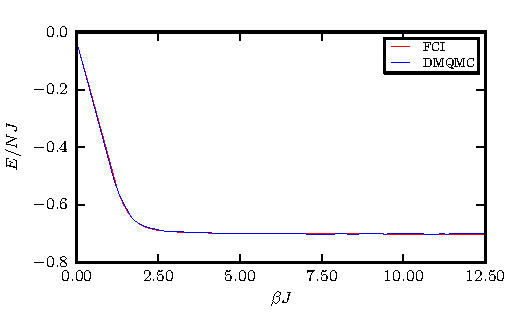
\includegraphics[width =1\textwidth]{4x4_nois_energy.pdf}
\caption[The DMQMC finite-temperature energy estimator for the $4\times4$ antiferromagnetic Heisenberg model.]{The DMQMC finite-temperature energy estimator (blue) and the exact FCI energy (red) for the $4\times4$ antiferromagnetic Heisenberg model. The DMQMC simulation ran with an initial population of $10^5$ psips and for $10^3$ $\beta$-loops. }
\label{fig:4x4_nois_energy}
\end{center}
\end{figure}
\begin{figure}[H]
\begin{center}
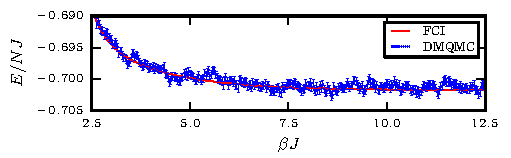
\includegraphics[width =1\textwidth]{4x4_energy_subplot.pdf}
\caption[The DMQMC energy estimator for the $4\times4$ antiferromagnetic Heisenberg model.]{The DMQMC finite-temperature energy estimator with statistical errors (blue) and the exact FCI energy (red) for the $4\times4$ antiferromagnetic Heisenberg model.}
\label{fig:4x4_nois_energy_subplot}
\end{center}
\end{figure}

A blocking analysis over a single $\beta$-loop yields a ground-state energy estimate of $E_0 = -0.7021(3)$, which is within error of the FCI ground-state energy\cite{SpencerFCI} of $E_0 = -0.7018$.

However, the number of psips used was larger than the size of the Hilbert space\footnote{But considerably less than the $1.7\times10^8$ elements of the density matrix}. So whilst the DMQMC results are reasonably accurate, the finite-temperature properties can be calculated with far less effort using FCI. For example, the DMQMC simulation running on 64 cores (2.8 Ghz) took approximately 3 hours to complete, whereas the FCI calculation took approximately 30 minutes on 2 cores (1.86 GHz). This could prove to be a problem with larger systems where even more psips are required.

\subsection{Staggered magnetisation}
The DMQMC finite-temperature squared staggered magnetisation estimator was also tested on the $4\times4$ antiferromagnetic Heisenberg model and the results are presented in Fig.~\ref{fig:4x4_nois_stag_mag} and  Fig.~\ref{fig:4x4_nois_stag_mag_subplot}. A blocking analysis over a single $\beta$-loop yields a ground-state squared staggered magnetisation estimate of $\langle (M^{\dagger})^2\rangle_0 = 0.2762(5)$, which agrees (within error) with the exact result of $\langle (M^{\dagger})^2\rangle_0 = 0.2765$ obtained by Dagotto and Moreo\cite{Dagotto1988} using a modified Lanczos method.
\begin{figure}[H]
\begin{center}
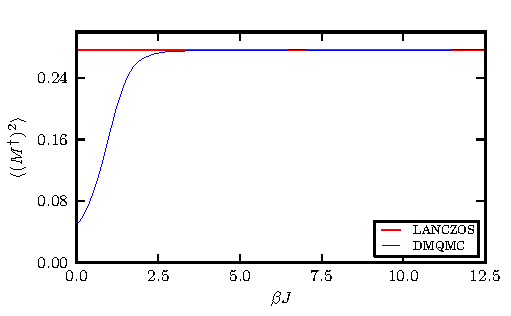
\includegraphics[width =1\textwidth]{4x4_nois_stag_mag.pdf}
\caption[The DMQMC finite-temperature squared staggered magnetisation estimator for the $4\times4$ antiferromagnetic Heisenberg model.]{The DMQMC finite-temperature squared staggered magnetisation estimator (blue) and the exact modified Lanczos ground-state squared staggered magnetisation (red) for the $4\times4$ antiferromagnetic Heisenberg model. The DMQMC simulation ran with an initial population of $10^5$ psips and for $10^3$ $\beta$-loops.}
\label{fig:4x4_nois_stag_mag}
\end{center}
\end{figure}
\begin{figure}[H]
\begin{center}
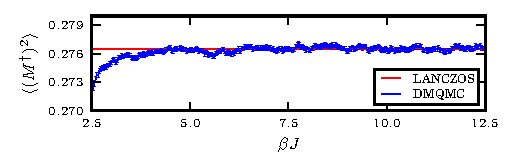
\includegraphics[width =1\textwidth]{4x4_stag_mag_subplot.pdf}
\caption[The DMQMC finite-temperature squared staggered magnetisation estimator with statistical errors for the $4\times4$ antiferromagnetic Heisenberg model.]{The DMQMC finite-temperature squared staggered magnetisation estimator with statistical errors (blue) and the exact modified Lanczos ground-state squared staggered magnetisation (red) for the $4\times4$ antiferromagnetic Heisenberg model.}
\label{fig:4x4_nois_stag_mag_subplot}
\end{center}
\end{figure}


\subsection{Heat capacity}
\label{sec:HeatCapacityResults}
Two methods for calculating the heat capacity in a constant magnetic field were introduced in Sec.~\ref{sec:heatCapacity}. One method was to calculate the derivative in Eq.~\ref{eq:splineDerivative} using a cubic spline fit of the finite-temperature energy estimator and the other was to directly sample the heat capacity during the DMQMC simulation. Both were tested on the $4\times4$ antiferromagnetic Heisenberg lattice with no magnetic field and are shown in Fig.~\ref{fig:4x4spline_spec_heat}. 

\begin{figure}[H]
\begin{center}
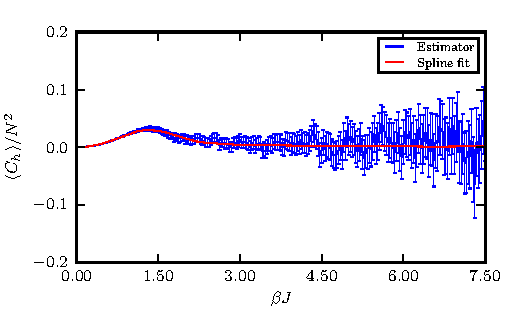
\includegraphics[width =1\textwidth]{4x4spline_spec_heat.pdf}
\caption[The heat capacity estimator calculated by the spline derivative method (red) and by direct stochastic sampling (blue) for a $4\times4$ antiferromagnetic Heisenberg lattice with no applied magnetic field]{The heat capacity estimator calculated by the spline derivative method (red) and by direct stochastic sampling (blue) for a $4\times4$ antiferromagnetic Heisenberg lattice.}
\label{fig:4x4spline_spec_heat}
\end{center}
\end{figure}

It was found that the spline fit method worked best. The direct stochastic sampling of the heat capacity suffered from huge fluctuations as $\beta$ grew large. This is due to the $\beta^2$ factor in Eq.~\ref{eq:heatCapacityEstimator}. As $\beta$ becomes large the fluctuations in $\langle H^2\rangle-\langle H\rangle^2$ are amplified resulting in heavy statistical noise. This is not the case for the other estimators studied, where the factor is absent. The spline fit on the $\langle H \rangle$ estimator smooths out the statistical fluctuations and removes the dependence on the $\langle H^2\rangle$ estimator, so performs better. Furthermore, the spline derivative method tends towards the correct value in the large $\beta$ limit. The heat capacity should be zero at absolute zero otherwise the third law of thermodynamics would be violated

\section{The $6\times6$ antiferromagnetic Heisenberg Lattice}
The Hilbert space of the $6\times6$ antiferromagnetic Heisenberg lattice contains a much larger $9.08\times10^9$ configurations in the $M_S = 0$ subspace. Although it is unfeasible to calculate exact FCI results for this system, it has been well-studied in the literature by methods such as GFQMC.

Fig.~\ref{fig:6x6_no_importance_sampling2_energy} shows the DMQMQ finite-temperature energy estimator fluctuating wildly after only a short range in $\beta$. It was not possible to obtain the ground-state energy. This simulation took roughly 10.5 hours on 64 cores (2.8 Ghz) and although the number of psips was only a fraction of the Hilbert space, DMQMC cannot be regarded as a competitive QMC algorithm unless some major improvements are found.
\begin{figure}[H]
\begin{center}
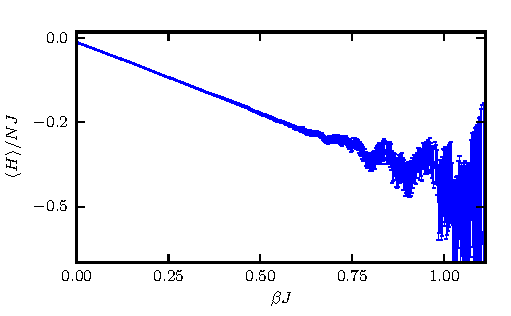
\includegraphics[width =0.82\textwidth]{6x6_no_importance_sampling2_energy.pdf}
\caption[The DMQMC finite-temperature energy estimator for the $6\times6$ antiferromagnetic Heisenberg model. ]{The DMQMC finite-temperature energy estimator for the $6\times6$ antiferromagnetic Heisenberg model.  The simulation ran with an initial population of $10^6$ psips and for $10^3$ $\beta$-loops.}
\label{fig:6x6_no_importance_sampling2_energy}
\end{center}
\end{figure}

\section{Importance sampling}
\label{sec:importanceSampling}

It was soon discovered that DMQMC was ineffective because the number of psips on the diagonal of the density matrix decays exponentially with inverse-temperature as shown in Fig.~\ref{fig:6x6_no_importance_sampling2_trace}. As psips spawn out from the diagonal and start to explore the complete space of density matrix elements, the chance of them spawning back onto the trace becomes very small. For example, psips that carry more than 1 excitation between their bitstring labels can no longer spawn directly back onto the diagonal, but have to do so in a number of steps. Meanwhile, the psips that were originally on the trace are killed off by the clone/death step of the DMQMC algorithm and so the population quickly diminishes. 
\begin{figure}[H]
\begin{center}
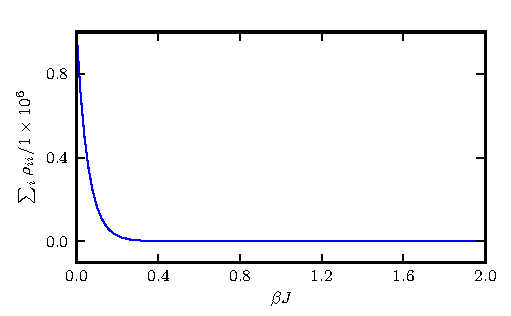
\includegraphics[width =1\textwidth]{6x6_no_importance_sampling2_trace.pdf}
\caption[Total number of psips on the trace as a function of $\beta$.]{Total number of psips on the trace as a function of $\beta$.}
\label{fig:6x6_no_importance_sampling2_trace}
\end{center}
\end{figure}

In order to improve the statistics on the trace at large $\beta$, spawning events onto the diagonal can be encouraged in a way that can be undone when calculating expectation value estimators. This can be achieved by increasing the probability of psips spawning onto the diagonal and assigning them a weight to be taken into account when calculating the estimators. More generally, to improve the statistics across all excitations, psips can either be encouraged or discouraged to spawn from one excitation to another and then assigned the relevant weight.

One can think of a scalar function $\mathcal{M}$, which maps an element of $\bm{\rho}$ to an element of a new matrix $\bm{\rho}'$, which evolves with improved statistics across all excitations. The scalar function takes as its arguments, the configurations $\ket{i}$ and $\ket{j}$ that represent the position of the element in $\bm{\rho}$ and the matrix element $\rho_{ij}$ itself. The function compares the two configurations and determines the number of excitations between them and hence scales the matrix element accordingly (equivalent to scaling the number of psips). So $\mathcal{M}$ can be thought of in the following way,
\begin{equation}
\rho'_{ij} = \mathcal{M}(\rho_{ij},\ket{i},\ket{j}) = W(\ket{i},\ket{j})\rho_{ij},
\label{eq:importanceSamplingTransformation}
\end{equation}
where $W$ is a scalar function that determines the excitation between $\ket{i}$ and $\ket{j}$ and returns the appropriate scaling factor. It is important to note that $W(\ket{i},\ket{j}) = W(\ket{j},\ket{i})$ as $\bm{\rho}$ is symmetric.

Now the inverse of $\mathcal{M}$ is obvious,
\begin{equation}
\mathcal{M}^{-1}(\ket{i},\ket{j},{\rho'}_{ij}) =  \frac{1}{W(\ket{i},\ket{j})}{\rho'}_{ij} = \rho_{ij}
\end{equation}

To make notation simple define
\begin{eqnarray}
\mathcal{M}({\rho}_{ij})  &\equiv& \mathcal{M}(\ket{i},\ket{j},\rho_{ij}) \\
\mathcal{M}^{-1}({\rho'}_{ij})  &\equiv& \mathcal{M}^{-1}(\ket{i},\ket{j},{\rho'}_{ij}) \\
W_{ij} &\equiv& W(\ket{i},\ket{j}).
\end{eqnarray}

Under this transformation the estimator for the expectation value of an operator, $O$, can be written
\begin{eqnarray}
\langle O \rangle = \frac{\sum_{i,j}\rho_{ij}O_{ji}}{\sum_{i}\rho_{ii}} &= & \frac{\sum_{i,j}\mathcal{M}^{-1}({\rho'}_{ij})O_{ji}}{\sum_{i}\mathcal{M}^{-1}({\rho'}_{ii})}\\
&=& \frac{\sum_{i,j}\frac{1}{W_{ij}}{\rho'}_{ij}O_{ji}}{\sum_{i}\mathcal{M}^{-1}({\rho'}_{ii})}\\
&=& W_{ii}\frac{\sum_{i,j}{\rho'}_{ij}\mathcal{M}^{-1}(O_{ji})}{\sum_{i}{\rho'}_{ii}}.
\label{eq:importanceSampledEstimator}
\end{eqnarray}
In the final step $\frac{1}{W_{ij}}O_{ji} = \mathcal{M}^{-1}(O_{ji})$ due to the symmetry of $W$ and the fact that $\bm{O}$ and $\bm{\rho}$ are expressed in the same basis. Moreover, $W_{ii}$ has been taken out of the summation because for each $i$ the excitation level is zero and hence $W_{ii}$ is constant.

So under the importance sampling transformation (Eq.~\ref{eq:importanceSamplingTransformation}), expectation value estimators can be obtained by applying the inverse transformation to the matrix $\bm{O}$, then taking the expectation value with respect to $\bm{\rho}'$ and finally multiplying by the weight given to the zeroth excitation. If the weights $W_{ij}$ are chosen carefully then the statistical error on the expectation value can be minimised.

\subsection{New population dynamics}

Given the importance sampling transformation (Eq.~\ref{eq:importanceSamplingTransformation}) it is possible to deduce a new set of rules for the population dynamics for the evolution of $\bm{\rho}'$, by transforming Eq.~\ref{eq:FirstOrderEuler},
\begin{multline}
\mathcal{M}^{-1}({\rho'}_{ij}(\beta +\Delta \beta)) = \\ \mathcal{M}^{-1}({\rho'}_{ij}(\beta))+\frac{1}{2}\sum_{m}\left(T_{im}\mathcal{M}^{-1}({\rho'}_{mj}(\beta))+\mathcal{M}^{-1}({\rho'}_{im}(\beta))T_{mj}\right)\Delta\beta.
\end{multline}
This simplifies to
\begin{equation}
{\rho'}_{ij}(\beta +\Delta \beta) = {\rho'}_{ij}(\beta)+\frac{1}{2}\sum_{m}\left(\frac{W_{ij}}{W_{mj}}T_{im}{\rho'}_{mj}(\beta)+{\rho'}_{im}(\beta)\frac{W_{ij}}{W_{im}}T_{mj}\right)\Delta\beta
\end{equation}

Therefore the rates at which psips spawn has changed so that they spawn from
\begin{equation}
\label{eq:ImportanceSpawningWeights}
(i,m)\to(i,j) \textnormal{\phantom{---}with probability\phantom{---}} \frac{W_{ij}}{2W_{im}}\lvert T_{mj} \rvert
\end{equation}
and from
\begin{equation}
\label{eq:ImportanceSpawningWeights2}
(m,j)\to(i,j) \textnormal{\phantom{---}with probability\phantom{---}} \frac{W_{ij}}{2W_{mj}}\lvert T_{im} \rvert.
\end{equation}
It is also important to note that when spawning in the opposite direction to in Eq.~\ref{eq:ImportanceSpawningWeights} and Eq.~\ref{eq:ImportanceSpawningWeights2} then the inverse weights must be applied.


\subsection{Choosing the weights}
An optimal set of weights can be chosen by studying the number of psips on each excitation level during a standard DMQMC run. Fig.~\ref{fig:excitations_nois} shows an example how the population of psips on each excitation changes as a function of $\beta$. In the ground-state some excitation levels are poorly sampled because they are occupied by small numbers of psips. 

\begin{figure}[H]
\begin{center}
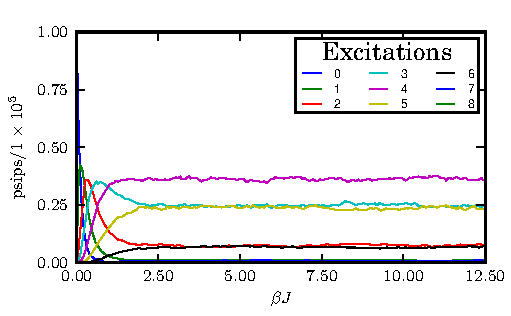
\includegraphics[width =1\textwidth]{excitations_nois.pdf}
\caption[The distribution of psips across the different excitation levels for a single $\beta$-loop of a DMQMC simulation of a $4\times4$ antiferromagnetic Heisenberg lattice.]{The distribution of psips across the different excitation levels for a single $\beta$-loop of a DMQMC simulation of a $4\times4$ antiferromagnetic Heisenberg lattice.}
\label{fig:excitations_nois}
\end{center}
\end{figure}
In the ground-state the number of psips on each excitation remains approximately constant. At this point the weights from Sec.~\ref{sec:importanceSampling} can be determined so that the total population of psips is distributed uniformly over the different excitation levels. For instance,
\begin{equation}
\label{eq:weightSelection}
W_n = \frac{N_{p}^{tot}}{N_{ex}N_p^{n}},
\end{equation}
where $W_n$ is the weight for the $n^{th}$ excitation, $N_p^{tot}$ is the total number of psips across all excitations,  $N_{ex}$ is the total number of excitations and $N_p^{n}$ is the total number of psips on the $n^{th}$ excitation.

When the importance sampling method was first tested, the weights were applied at the start of the simulation as shown in Fig~\ref{fig:excitations_is_instant}. 
\begin{figure}[H]
\begin{center}
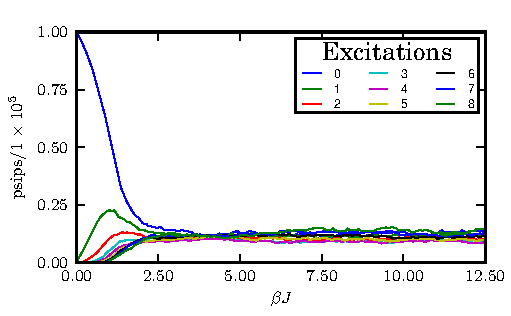
\includegraphics[width =1\textwidth]{excitations_is_instant.pdf}
\caption[The distribution of psips across the different excitation levels for a single $\beta$-loop of a DMQMC simulation of a $4\times4$ antiferromagnetic Heisenberg lattice, with importance sampling weights fully applied at $\beta = 0$.]{The distribution of psips across the different excitation levels for a single $\beta$-loop of a DMQMC simulation of a $4\times4$ antiferromagnetic Heisenberg lattice, with importance sampling weights fully applied at $\beta = 0$.}
\label{fig:excitations_is_instant}
\end{center}
\end{figure} It is evident that initially spawning events from the diagonal are restricted leading to an effective truncation of the Hilbert space as other excitations are suppressed. This meant that the higher excitations were being under-sampled for the initial evolution, which lead to biased results.

The weights were then introduced gradually, as shown in Fig.~\ref{fig:excitations_is}, so that in the ground-state ($\beta > \beta_{gs}$) they had reached the intended values. Each weight, $W$, was set to unity at $\beta = 0$ and for each step of $\Delta \beta$ they were scaled by $W^{\frac{\Delta\beta}{\beta_{gs}}}$ so that for $\beta > \beta_{gs}$ the weights were fully applied. Gradually introducing the weights in this way avoided a discontinuity in the spawning probabilities, whilst also reducing the effective truncation of the Hilbert space.  In this way, the psip populations in the pre-ground-state evolution is more similar to the case where no importance sampling is applied (Fig.~\ref{fig:excitations_nois}).

\begin{figure}[H]
\begin{center}
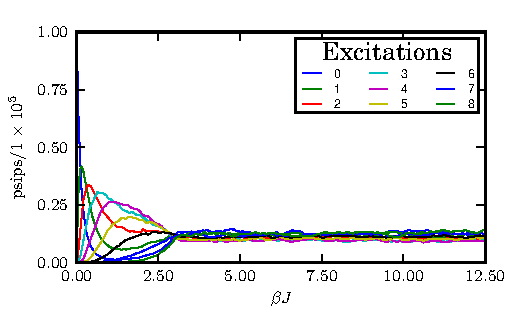
\includegraphics[width =1\textwidth]{excitations_is.pdf}
\caption[The distribution of psips across the different excitation levels for a single $\beta$-loop of a DMQMC simulation of a $4\times4$ antiferromagnetic Heisenberg lattice, with the importance sampling weights introduced gradually.]{The distribution of psips across the different excitation levels for a single $\beta$-loop of a DMQMC simulation of a $4\times4$ antiferromagnetic Heisenberg lattice, with the importance sampling weights introduced gradually. }
\label{fig:excitations_is}
\end{center}
\end{figure}

\subsection{Importance sampling implementation}
This method of importance sampling is simple to implement. When attempting to spawn, as in Eq.~\ref{eq:ImportanceSpawningWeights}, the excitation level of the current density matrix element can be found by performing a bit-wise \texttt{XOR} between the two bistrings that label it. The number of bits that are set in the output is equal to the number of excitations between the two bitstrings. This operation can also be used to determine the number of excitations between the two bitstrings labelling the density matrix element that a psip is spawning to. It is then easy to apply the correct weight to the spawning probability using Eq.~\ref{eq:ImportanceSpawningWeights}.

When adding the contribution from a particular density matrix element to the estimator, the above weighting can be undone easily by calculating the excitation level between the two labelling bit strings (using the bit-wise \texttt{XOR} operation) and then dividing by the corresponding weight.

\section{The $6\times6$ antiferromagnetic Heisenberg lattice revisited}
Now that an importance sampling method has been established, the $6\times6$ antiferromagnetic Heisenberg model can be re-investigated. 
\subsection{Energy}
The importance-sampled DMQMC energy estimator is shown in Fig~\ref{fig:6x6_10000000_6_energy} and with errors in Fig~\ref{fig:6x6_10000000_6_energy_subplot}. It shows a dramatic improvement in performance over standard DMQMC and with considerably less sampling. The energy now converges towards a reasonable value for the ground-state energy. For example, a blocking analysis of the DMQMC energy estimator yielded a ground-state energy of $E_0 = -0.6781(5)$, compared to Runge's GFQMC ground-state energy\cite{Runge1992} of $E_0 = -0.678871(8)$. An interesting point to note is that in this case the initial number of psips occupy only $1.21\times10^{-13}$ of the elements of the density matrix, so the performance improvement is huge.

\subsection{Staggered magnetisation}

The importance-sampled DMQMC squared staggered magnetisation estimator is shown in Fig~\ref{fig:6x6_10000000_6_energy}. The squared staggered magnetisation estimator converges to the ground-state value of $\langle (M^{\dagger})^2\rangle_0 = 0.2098(2)$, which was found via a blocking analysis of a single $\beta$-loop. This agrees with the value of $\langle (M^{\dagger})^2\rangle_0 = 0.20986(8)$ that was calculated by Runge using GFQMC\cite{Runge1992a}.

\begin{figure}[H]
\begin{center}
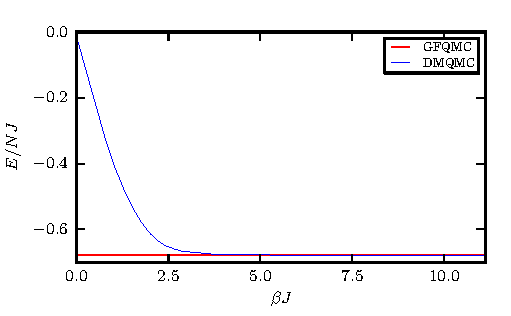
\includegraphics[width =1\textwidth]{6x6_10000000_6_energy.pdf}
\caption[The DMQMC finite-temperature energy estimator with importance sampling for the $6\times6$ antiferromagnetic Heisenberg model]{The DMQMC finite-temperature energy estimator with importance sampling (blue) and an accurate GFQMC estimate for the ground-state energy (red) for the $6\times6$ antiferromagnetic Heisenberg model. The simulation ran with an initial population of $1\times10^7$ psips and for $6$ $\beta$-loops. }
\label{fig:6x6_10000000_6_energy}
\end{center}
\end{figure} 
\begin{figure}[H]
\begin{center}
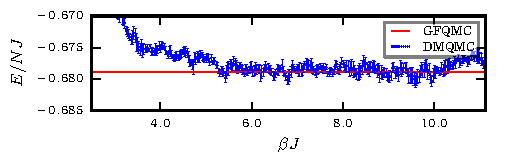
\includegraphics[width =1\textwidth]{6x6_10000000_6_energy_subplot.pdf}
\caption[The importance-sampled DMQMC finite-temperature energy estimator with statistical errors for the $4\times4$ antiferromagnetic Heisenberg model.]{The importance-sampled DMQMC finite-temperature energy estimator with statistical errors (blue) and an accurate GFQMC estimate for the ground-state energy (red) for the $4\times4$ antiferromagnetic Heisenberg model. }
\label{fig:6x6_10000000_6_energy_subplot}
\end{center}
\end{figure}

\begin{figure}[H]
\begin{center}
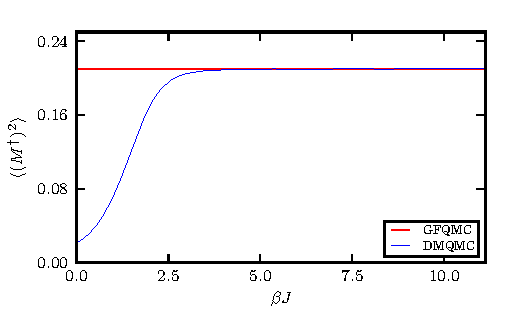
\includegraphics[width =1\textwidth]{6x6_10000000_6_stag_mag.pdf}
\caption[The DMQMC finite-temperature squared staggered magnetisation estimator with importance sampling for the $6\times6$ antiferromagnetic Heisenberg model.]{The DMQMC finite-temperature squared staggered magnetisation estimator with importance sampling (blue) and an accurate GFQMC estimate for the ground-state squared staggered magnetisation (red) for the $6\times6$ antiferromagnetic Heisenberg. The simulation ran with an initial population of $10^7$ psips and for $6$ $\beta$-loops.}
\label{fig:6x6_10000000_6_stag_mag}
\end{center}
\end{figure}
\begin{figure}[H]
\begin{center}
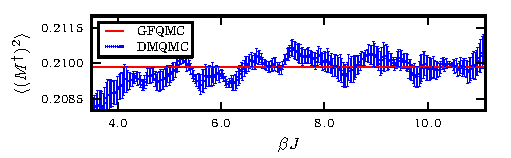
\includegraphics[width =1\textwidth]{6x6_10000000_6_stag_mag_subplot.pdf}
\caption[The importance-sampled DMQMC finite-temperature squared staggered magnetisation estimator with statistical errors or the $6\times6$ antiferromagnetic Heisenberg model.]{The importance-sampled DMQMC finite-temperature squared staggered magnetisation estimator with statistical errors (blue) and an accurate GFQMC estimate for the ground-state square staggered magnetisation (red) for the $6\times6$ antiferromagnetic Heisenberg model. }
\label{fig:6x6_10000000_6_stag_mag_subplot}
\end{center}
\end{figure}
%\subsection{Heat capacity}
%\begin{figure}[H]
%\begin{center}
%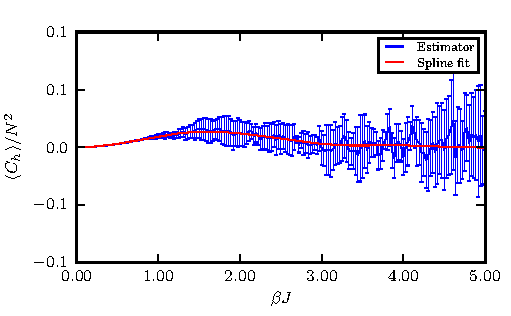
\includegraphics[width =1\textwidth]{6x6spline_spec_heat.pdf}
%\caption{}
%\label{fig:6x6spline_spec_heat}
%\end{center}
%\end{figure}

\section{The $4\times4\times4$ antiferromagnetic Heisenberg lattice}
The importance-sampled DMQMC algorithm was also tested on the $4\times4\times4$ antiferromagnetic Heisenberg lattice and the results are shown in Fig.~\ref{fig:4x4x4_is_energy} and Fig.~\ref{fig:4x4x4_is_energy_subplot}. It was difficult to test the accuracy of the DMQMC method in three dimensions, as the three dimensional antiferromagnetic Heisenberg model features less prominently in the literature. Nevertheless, the DMQMC ground-state energy estimate was compared against an accurate ground-state energy estimate obtained via FCIQMC\cite{SpencerFCIQMC}. 

Performing a blocking analysis, on a single $\beta$-loop DMQMC simulation gives a ground-state energy of $E_0 = -0.912(6)$, whereas a single run of the FCIQMC algorithm\cite{SpencerFCIQMC} gives a ground-state energy of $E_0 = -0.91509(5)$. The FCIQMC value was obtained using an initial population of $10^6$ psips. DMQMC seems a good compromise between accuracy and the ability to obtain finite-temperature estimates.

The Hilbert space for a $4 \times 4 \times 4$ lattice contains roughly $1.83\times10^{18}$ spin configurations and so in this case DMQMC was simulating a density matrix with approximately $1.83\times10^{36}$ elements using only $5\times10^5$ psips. The statistical errors in Fig.~\ref{fig:4x4x4_is_energy_subplot} are surprisingly small considering the number of psips used.

\begin{figure}[H]
\begin{center}
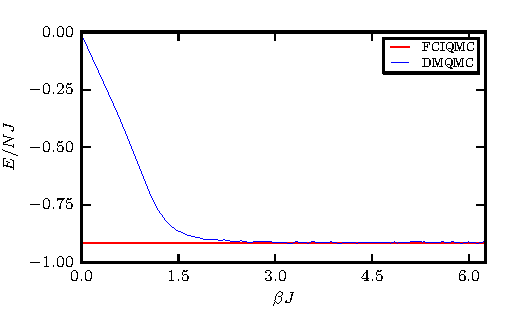
\includegraphics[width =1\textwidth]{4x4x4_is_energy.pdf}
\caption[The DMQMC finite-temperature energy estimator with importance sampling for the $4\times4\times4$ antiferromagnetic Heisenberg model.]{The DMQMC finite-temperature energy estimator with importance sampling (blue) and an accurate FCIQMC estimate for the ground-state energy (red) for the $4\times4\times4$ antiferromagnetic Heisenberg model.  The simulation ran with an initial population of $5\times10^6$ psips and for $43$ $\beta$-loops.}
\label{fig:4x4x4_is_energy}
\end{center}
\end{figure}
\begin{figure}[H]
\begin{center}
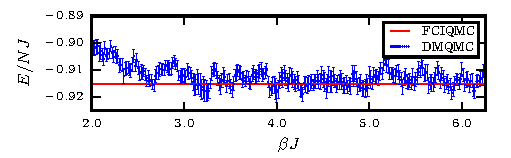
\includegraphics[width =1\textwidth]{4x4x4_is_energy_subplot.pdf}
\caption[The importance-sampled DMQMC finite-temperature energy estimator with statistical errors for the  $4\times4\times4$ antiferromagnetic Heisenberg model.]{The importance-sampled DMQMC finite-temperature energy estimator with statistical errors (blue) and an accurate FCIQMC estimate for the ground-state energy (red) for the $4\times4\times4$ antiferromagnetic Heisenberg model.}
\label{fig:4x4x4_is_energy_subplot}
\end{center}
\end{figure}

\section{Summary}
The DMQMC implementation was tested on some simple antiferromagnetic Heisenberg models in both two and three dimensions. With the standard algorithm, developed in Ch.~\ref{ch:chapter1}, it was found that the initial population of psips was similar to the size of the Hilbert space of configurations and failed for larger systems. It appeared as though the method might not be efficient enough to compete as a QMC method. 

However, the reason for this poor performance was soon realised and a suitable importance sampling adaptation to the algorithm was invented, giving dramatically improved results. This new method allowed for accurate finite-temperature calculations of energy and staggered magnetisation for the $6\times6$ Heisenberg lattice, for which the conventional DMQMC method had failed. Importance sampling also enabled accurate simulation of the $4\times4\times4$ antiferromagnetic Heisenberg model. In most cases the DMQMC ground-state estimators (obtained via a blocking analysis) were equal to the results in the literature, within error.

Additionally, both versions of the heat capacity estimator were tested on the $4\times4$ antiferromagnetic Heisenberg lattice. It was found that directly sampling the heat capacity from the DMQMC simulation gave poor results, even with importance sampling. This was because the statistical fluctuations were amplified for large $\beta$. This proved the point that, although in DMQMC it is theoretically possible to calculate the expectation value of any quantum mechanical operator, in practice it can prove to be difficult to obtain accurate results. The spline derivative method did provide improved results, but this method requires post-processing of the data and makes it difficult to determine errors. 

%%% Local Variables: 
%%% mode: latex
%%% TeX-master: "../thesis"
%%% End: 

\chapter{Application to Quantum Information}
\label{ch:chapter3}
\ifpdf
    \graphicspath{{Chapter3/Chapter3Figs/PNG/}{Chapter3/Chapter3Figs/PDF/}{Chapter3/Chapter3Figs/}}
\else
    \graphicspath{{Chapter3/Chapter3Figs/EPS/}{Chapter3/Chapter3Figs/}}
\fi

Entanglement is the fundamental inseparability of quantum systems - seen as correlations that emerge in quantum theory and that cannot be described by classical physics. It has been described as ``the strangest and least understood facet of quantum theory''\cite{Rudolph} and this, in itself, provides a good motivation for the study of quantum entanglement. Furthermore, some future technologies such as quantum computers, quantum teleportation and ion clocks\cite{Rudolph} rely on the unique properties of entanglement. A method that can calculate measures of entanglement between qubits or systems of qubits could prove useful in the development of such technologies. 

Currently, there are no known scalable simulation methods\cite{Hastings2010} that are capable of calculating entanglement measures. Entanglement simulations rely on non-scalable algorithms such as density matrix renormalisation group (DMRG) or Lanczos. Other QMC methods do not provide access to the reduced density matrix. However, with DMQMC and the stochastic sampling of the full density matrix, it is possible to obtain the reduced density matrix.

This chapter begins by introducing the two main measures of entanglement (concurrence and Von-Neumann entropy) in quantum information theory. It moves on to discuss how estimators for such methods can be incorporated into the DMQMC algorithm. Finally, the estimator for concurrence is tested against some simple 1D antiferromagnetic Heisenberg rings in the presence and absence of an applied magnetic field.

\section{Reduced Density Matrix}

A major obstacle that prevents QMC simulations of entanglement measures in many-electron quantum systems is the difficulty of obtaining the reduced density matrix. In DMQMC, it is possible to obtain a reduced density matrix for a small subsystem (small enough so that it can be stored and manipulated in computer memory).

Consider two quantum systems $A$ and $B$ that are coupled to form a system $C$ (Fig.~\ref{fig:coupledSubsystems}) such that
\begin{equation}
\mathcal{H}_C = \mathcal{H}_A \otimes \mathcal{H}_B,
\label{eqn:coupledSubsystems}
\end{equation}
where $\mathcal{H}_A$, $\mathcal{H}_B$ and $\mathcal{H}_C$  denote the Hilbert spaces of systems $A$, $B$ and $C$. 
\begin{figure}[H]
\begin{center}

\includegraphics[width =0.49\textwidth]{subsystems.pdf}
\caption{Two quantum systems, $A$ and $B$ coupled such that the quantum state of the complete system lives in a Hilbert space that is the tensor product of the Hilbert spaces of $A$ and $B$.}
\label{fig:coupledSubsystems}
\end{center}
\end{figure}

\noindent In the Schmidt basis\cite{Knight1994} a quantum state, $\ket{\psi}$, of system $C$ can be expressed in terms of the basis vectors of systems $A$ and $B$,
\begin{equation}
\ket{\psi} = \sum_{n}\alpha_{n}\ket{a_n}\otimes\ket{b_n}.
\end{equation}
With $\ket{a_n}\in\mathcal{H}_A$ and $\ket{b_n}\in\mathcal{H}_B$. Now consider taking a measurement, $O_A$, on system $A$ without touching $B$, the expected outcome of this measurement is then,
\begin{eqnarray}
\bra{\psi}O_A \otimes \mathbb{1}_B\ket{\psi} &=& \bra{\psi} \sum_{n}\alpha_n O_A\ket{a_n}\otimes\ket{b_n} \\ &=& \sum_{n,m}\alpha_m^*\alpha_n\bra{a_m} O_A \ket{a_n}\otimes\langle b_m | b_n\rangle
\\ &=& \sum_n \lvert\alpha\rvert^2\bra{a_n} O_A \ket{a_n} \\
&=& \textnormal{Tr}_A(\rho_A O_A),
\end{eqnarray}
where $\mathbb{1}_B$ is the identity operator acting on system $B$, $\rho_A$ is the reduced density operator\footnote{it satisfies the three properties in Sec.~\ref{sec:DensityMatrix}} for system $A$ and $\textnormal{Tr}_A$ is the partial trace over the basis of system $B$. The reduced density operator, $\rho_A$ may be obtained by ``tracing out'' system $B$ from the projector onto state $\ket{\psi}\in\mathcal{H}_C$ i.e.

\begin{eqnarray}
\rho_C &=& \ket{\psi}\bra{\psi} = \sum_{n,m}\alpha_n\alpha_m^*\ket{a_n}\bra{a_m}\otimes\ket{b_n}\bra{b_m}\\
\rho_A &=& \textnormal{Tr}_B(\rho_C) = \sum_{n,m}\alpha_n\alpha_m^*\ket{a_n}\bra{a_m}\otimes\textnormal{Tr}(\ket{b_n}\bra{b_m})\\
&=&\sum_n \lvert \alpha\rvert^2 \ket{a_n} \bra{a_n}.
\label{eq:traceOut}
\end{eqnarray}
So in DMQMC, it is also possible to stochastically sample the reduced density matrix for a subsystem of the total system under study. From this it is possible to calculate expectation values for measurement on that subsystem. Moreover, it allows for some interesting measures of quantum entanglement between the subsystems $A$ and $B$.
% ------------------------------------------------------------------------

\section{Von-Neumann Entropy}

The Von-Neumann Entropy is an extension of the Shannon entropy, from classical information theory into quantum information theory. In classical information theory, the Shannon entropy for a probability distribution $q_1,\dots, q_n$ is 
\begin{equation}
S_C(q_1,\dots,q_n)=\sum_i q_i \log_2 1/q_i.
\end{equation}
Similarly for a quantum state living in a finite $D$-dimensional Hilbert space, the Von-Neumann entropy is
\begin{equation}
\label{eq:VonNeumannEntropy}
S_Q(\bm{\rho}) = -\textnormal{Tr}(\bm{\rho}\log_2\bm{\rho}) = \sum_i p_i \log_2 1/p_i,
\end{equation}
where $p_i$ are the eigenvalues of $\bm{\rho}$. It describes the purity of the system. If one considers the density matrix in diagonal form, the eigenvalues $p_i$ represent the probability of the system being in some state $\ket{i}$ of the diagonal basis. Hence, for a pure state one eigenvalue is unity, whilst all the others are zero, giving a zero Von-Neumann entropy. However, for a maximally entangled mixed state, with equally likely probabilities of being in any of the states $\ket{i}$ in the diagonal basis, the Von-Neumman entropy is $\log_2{D}$. 

Therefore, if the Von-Neumann entropy is calculated for the reduced density matrix for system $A$, in Fig.~\ref{fig:coupledSubsystems}, it measures the amount of quantum entanglement between systems $A$ and $B$. For example, if the Von-Neumann entropy is zero, then $A$ is a pure state and so there is no entanglement between $A$ and $B$, assuming that the overall system $C$ is in a pure state. On the other hand if the Von-Neumann entropy is $\log_2{D}$, then subsystem $A$ is in a fully mixed state and $A$ and $B$ must be maximally entangled.

In order to compute the Von-Neumann entropy (Eq.~\ref{eq:VonNeumannEntropy}), the subsystem $A$ must be sufficiently small so that the reduced density matrix can be diagonalised directly. The Von-Neumann entropy has not been properly tested due to time restrictions. 

% ------------------------------------------------------------------------

\section{Concurrence and Entanglement of Formation}

In 2001, Hill and Wootters~\cite{Hill1997} introduced a new measure of entanglement for a two-qubit mixed state. For the case where the total system is mixed, the Von-Neumann entropy is no longer a good measure of quantum entanglement, because both subsystems $A$ and $B$ can have non-zero entropy even if there is no entanglement. The measure, known as the ``entanglement of formation'' is a generalisation of Von-Neumann entropy. The entanglement of formation of a bipartite quantum system can be defined as ``the minimum number of singlets needed to create an ensemble of pure states that represents a mixed state''~\cite{Wootters2001}. In this case a ``singlet'' refers to a state with zero total spin. 

Another definition of the Von-Neumann entropy, $E(\Phi)$, is the number of singlet pairs, required to required to create a copy of a pure state $\ket{\Phi}$\cite{Wootters2001}.The number of singlets required to create a copy of some mixed state that is expressed as an ensemble of pure states, $\rho = \sum_{j=1}^N p_j\ket{\Phi_j}\bra{\Phi_j}$, can be written
\begin{equation}
N_s = \sum_{j=1}^N p_jE(\Phi_j).
\end{equation}
This number depends on the particular ensemble so the minimum over all pure-state decompositions is taken in order to pick out the irreducible entanglement of the mixed system
\begin{equation}
E_f(\rho) = \min\left( \sum_{j}^N p_jE(\Phi_j) \right).
\end{equation}

For the special case of a two-qubit mixed state the entanglement of formation can be calculated from a quantity known as ``concurrence''. For a reduced density matrix, $\bm{\rho}_A$, where in this case $A$ refers to a subsystem of two qubits, the concurrence is defined as
\begin{equation}
\mathcal{C}(\bm{\rho}_A) \equiv \textnormal{max}(0, \gamma_1-\gamma_2-\gamma_3-\gamma_4),
\end{equation}
in which $\gamma_1 > \gamma_2 > \gamma_3 > \gamma_4$ are the eigenvalues of the matrix
\begin{equation}
\bm{R} = \sqrt{\sqrt{\bm{\rho}_A}\tilde{\bm{\rho}}_A\sqrt{\bm{\rho}_A}} \textnormal{\phantom{---}with\phantom{---}}  \tilde{\bm{\rho}}_A = (\sigma_y\otimes\sigma_y)\bm{\rho}_A^*(\sigma_y\otimes\sigma_y),
\end{equation}
where $\sigma_y$ is the Pauli spin matrix for the $y$-direction.

The concurrence, $\mathcal{C}$, ranges from zero to one and is monotonically related to the entanglement of formation~\cite{Hill1997}. In this way the concurrence can also be regarded as a measure of entanglement. The entanglement of formation for two qubits~\cite{Wootters2001} is given by,
\begin{equation}
\mathcal{E}(\mathcal{C}) = h\left( \frac{1+\sqrt{1-\mathcal{C}^2}}{2}\right)
\textnormal{\phantom{---}with\phantom{---}}
h(x) = -x\log_2 x - (1-x)\log_2 (1-x).
\end{equation}

The concurrence is easy to compute for the Heisenberg model. If it is assumed that the Hamiltonian is real (as is the case in the Heisenberg model) and therefore that the reduced density matrix is also real, the problem is reduced to finding the moduli of the eigenvalues of 
\begin{equation}
\label{eq:concurrenceMatrix}
\tilde{\bm{R}} = \bm{\rho}_A(\sigma_y\otimes\sigma_y).
\end{equation}
As $\tilde{\bm{R}}$ is only a $4\times4$ matrix it is trivial to compute the concurrence.
% ------------------------------------------------------------------------
\section{Implementation of the ground-state entanglement estimators}
Whilst it is possible to calculate finite-temperature estimators for both the Von-Neumann entropy and Concurrence, the current implementation can only handle such estimators for the ground-state. This is because   the current implementation is based on previous FCIQMC code which only allows simulations for a single $M_S$ subspace. In FCIQMC the ground-state always lies within a known $M_S$. For example, in a simulation for the antiferromagnetic Heisenberg model with zero applied magnetic field the ground-state is within the $M_S=0$ subspace. Unfortunately, there was not enough time during this MSci project to adapt the code so that simulations could run in all subspaces simultaneously, which would allow for finite-temperature estimators of entanglement.

In the current implementation the reduced density matrix, for a specified subsystem of spins, is averaged over all $\beta>\beta_{gs}$, where $\beta_{gs}$ is the critical $\beta$ beyond which the simulation enters the ground-state. This is to ensure that the reduced density matrix has the highest possible accuracy before computing the entanglement estimators.

In order to obtain the reduced density matrix at a particular $\beta > \beta_{gs}$ the subsystem $B$ is traced out as in Eq.~\ref{eq:traceOut}. This was achieved by looping over all elements of the total density matrix with non-zero psip populations and determining whether a particular element contributed towards the reduced density matrix. A simple test (see Fig.~\ref{fig:rdm_algorithm}) was devised to determine whether this was the case:

\begin{enumerate}
\item Define a boolean mask for subsystem $B$ - this is created at the start of the simulation and has bits set to 1 where a spin is to be included in subsystem $B$.
\item Perform a bit-wise \texttt{AND} operation on each of the two bit string ends that label the current density matrix element, with the boolean mask for subsystem $B$. This sets all bits that represent a spin in subsystem $A$ to 0 and leave those that represent a spin in $B$ unchanged.
\item If the two resultant bit strings are equal then this means that it lies on the diagonal of subsystem $B$ and hence contributes to the reduced density matrix for subsystem $A$. In this case, the psip charge on this element is added to the corresponding element of the reduced density matrix. If they are not equal then nothing is added to the reduced density matrix.
\end{enumerate}

\begin{figure}[H]
\begin{center}
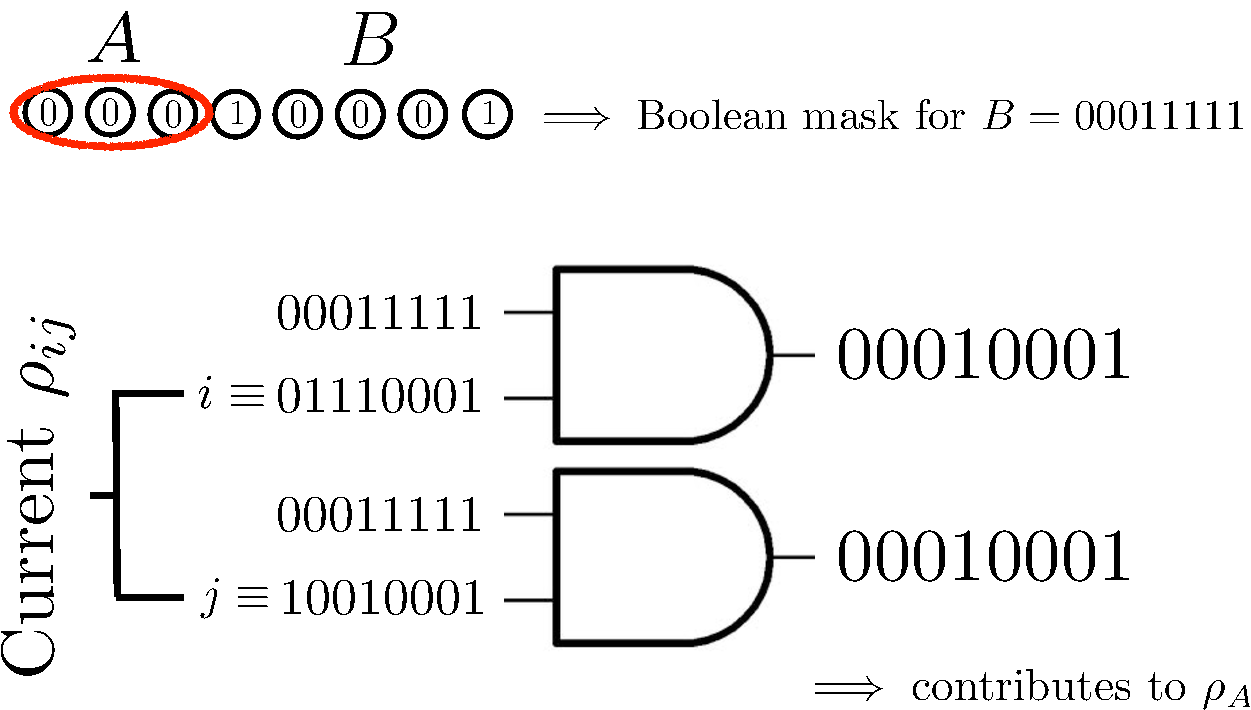
\includegraphics[width =0.8\textwidth]{rdm_algorithm.pdf}
\caption{Illustration of how a given density matrix element $\rho_{ij}$ is tested to see whether it contributes towards $\rho_A$ for the case that $A$ is 3 neighbouring spins on a chain of length $N=8$}
\label{fig:rdm_algorithm}
\end{center}
\end{figure}

After obtaining the average reduced density matrix, the Von-Neumann entropy is obtained by directly diagonalising the reduced density matrix\footnote{This is achieved using the \texttt{LAPACK ssyev} and \texttt{dsyev} routines for diagonalising symmetric matrices. These routines use the QR algorithm.}. For the concurrence, the matrix $\tilde{R}$ (Eq.~\ref{eq:concurrenceMatrix}) is diagonalised\footnote{This is achieved using the \texttt{LAPACK sgeev} and \texttt{dgeev} routines for diagonalising nonsymmetric matrices. Both routines first use Hessenberg reduction followed by the QR algorithm.}. This whole process is repeated over multiple $\beta$-loops to build up statistics and to enable the calculation of errors as in Sec.~\ref{sec:statErrCalc}.
% ------------------------------------------------------------------------
\section{Nearest-neighbour concurrence in Heisenberg rings}
The ground-state concurrence for neighbouring spins (qubits), illustrated in Fig.~\ref{fig:HeisenbergRing}, on a bipartite antiferromagnetic Heisenberg ring with $N$ qubits was first calculated by O'Connor and Wooters in 2001\cite{OConnor2001}. They found that the ground-state concurrence, $\mathcal{C}_{gs}$, is related to the ground-state energy, $E_{0}$, in the following way
\begin{equation}
\label{eq:groundstateConcurrence}
\mathcal{C}_{gs} = -\frac{1}{2}(E_{0}/N + 1).
\end{equation}

\begin{figure}[h!]
\begin{center}
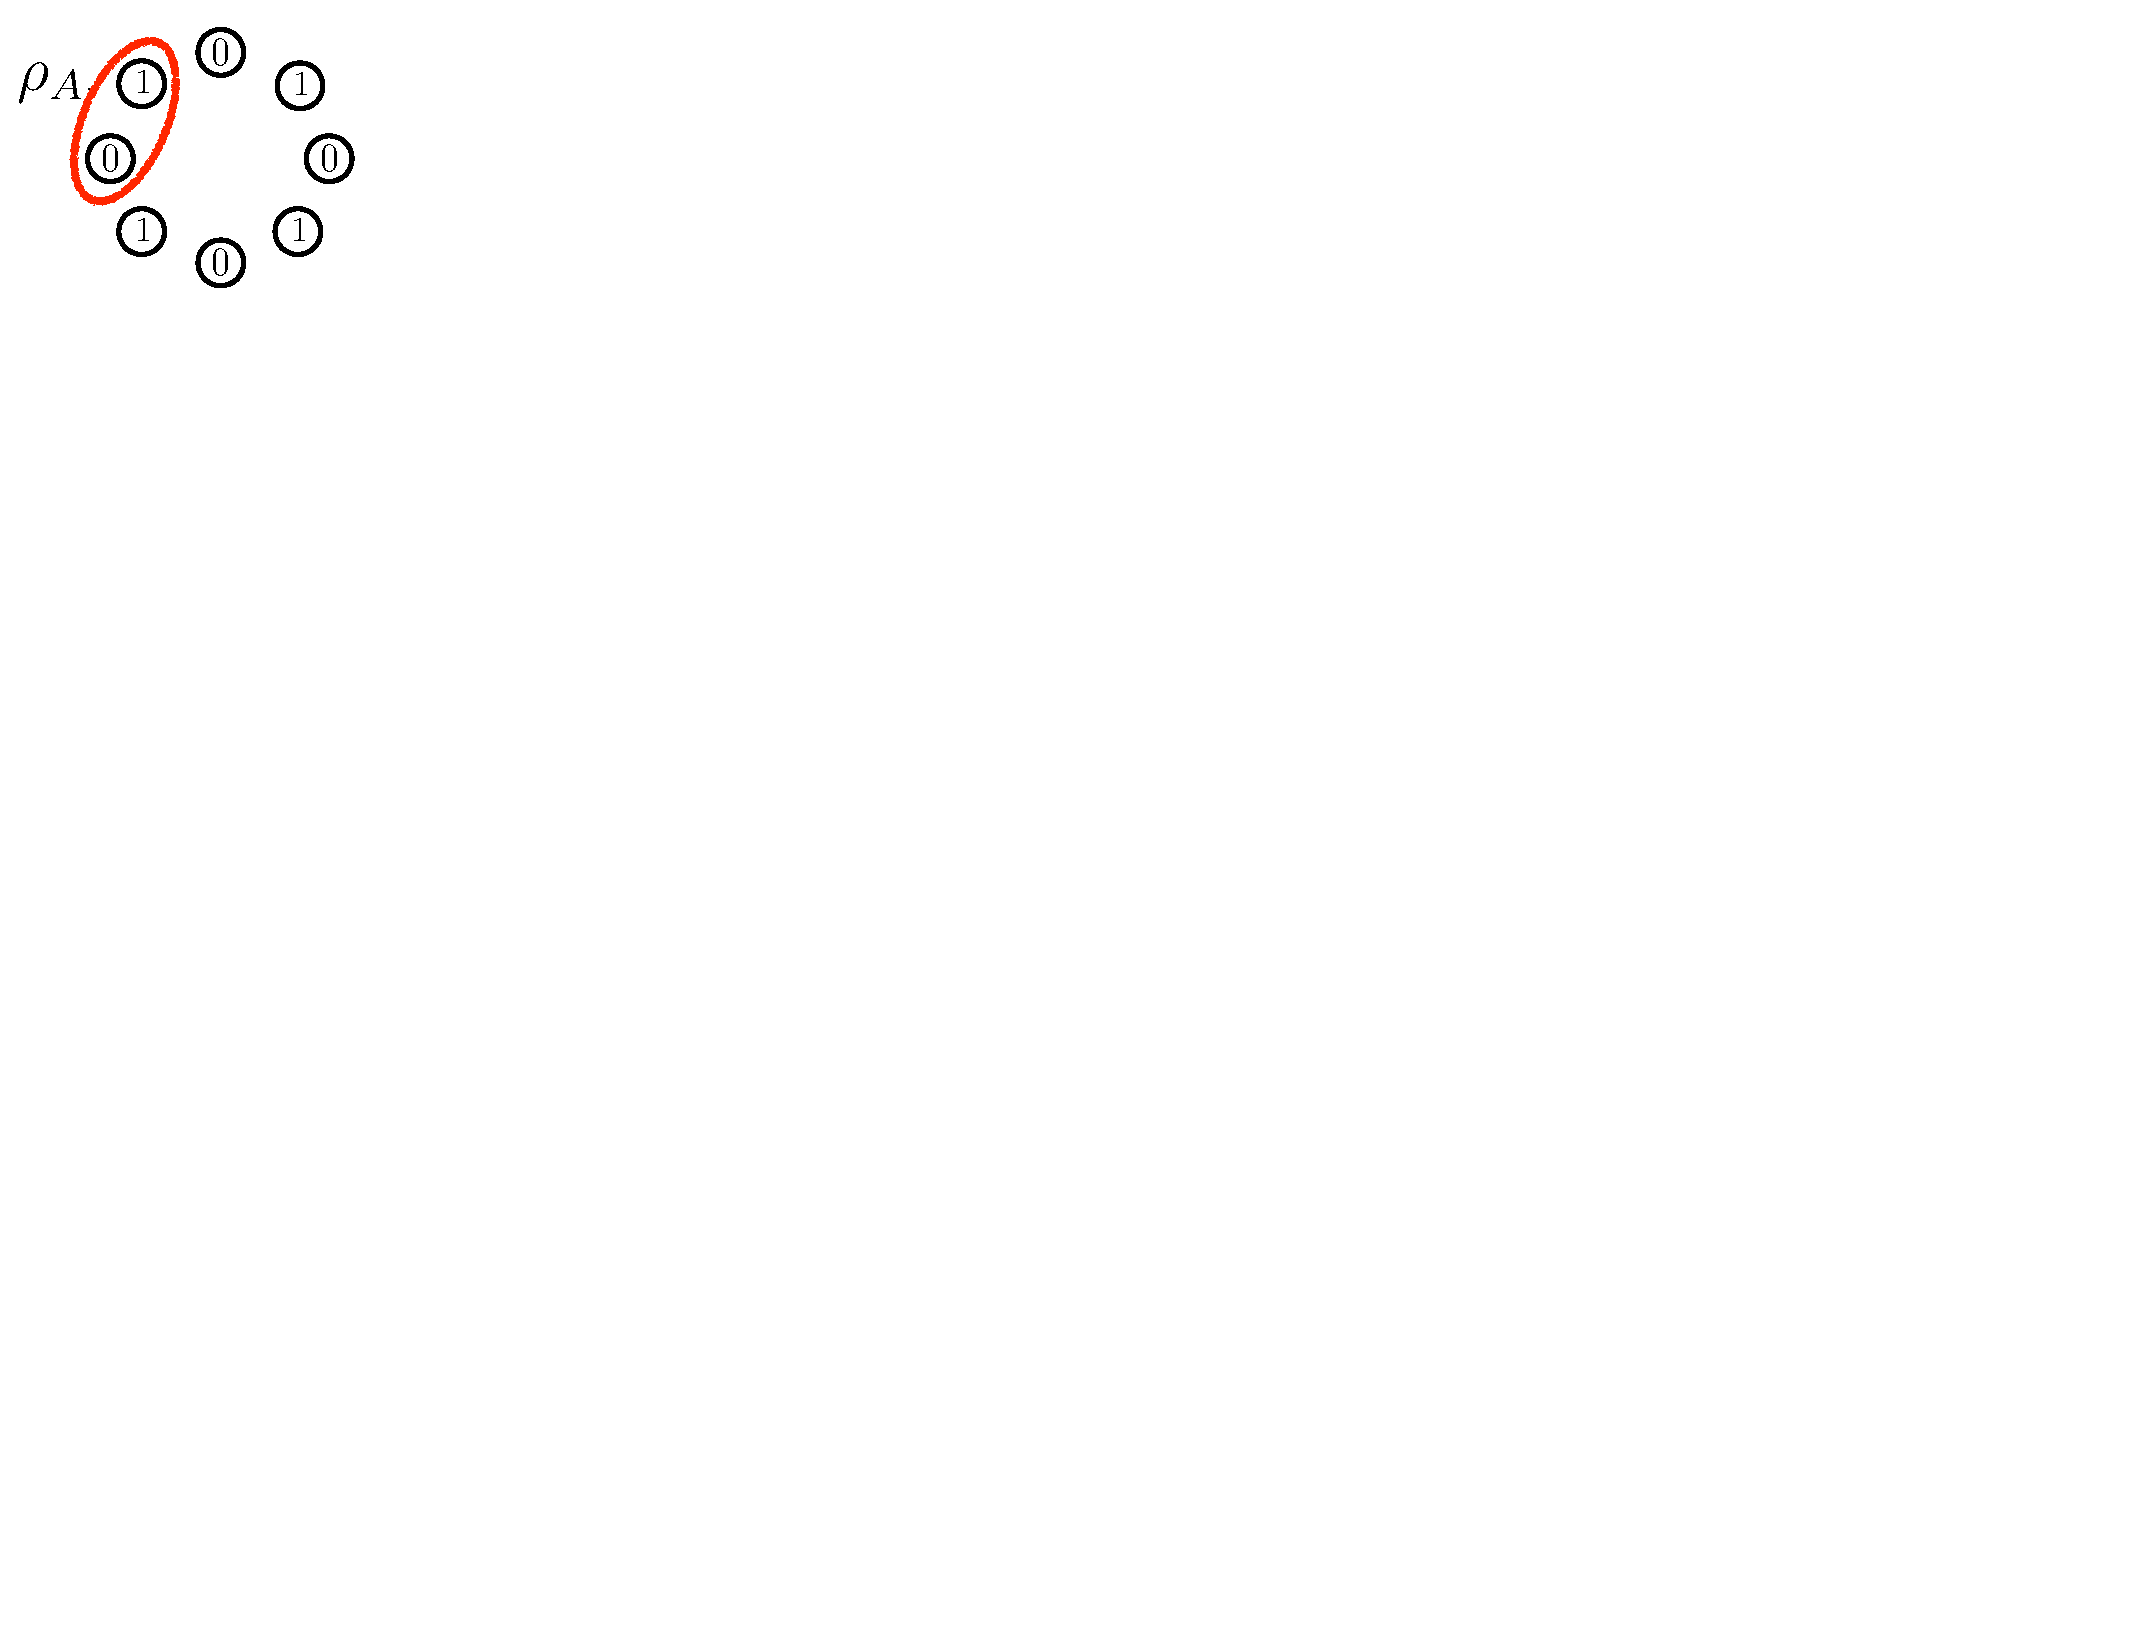
\includegraphics[width =0.49\textwidth]{HeisenbergRing.pdf}
\caption{Illustration of the subsystem of two qubits, $A$, on an $N = 8$ antiferromagnetic Heisenberg chain. The system can be regarded as a ring due to the periodic boundary conditions adopted.}
\label{fig:HeisenbergRing}
\end{center}
\end{figure}

To test whether the DMQMC ground-state concurrence estimator was implemented correctly, several Heisenberg rings of differing size were simulated. The results in Tab. 4.1, show that the DMQMC ground-state concurrence estimator was correct within error for bipartite rings up to $N=10$. Moreover, an $N=36$ Heisenberg ring was simulated with importance sampling and the ground-state concurrence of $\mathcal{C}_{gs} = 0.3873(8)$ was obtained. This agrees well with the value of $\mathcal{C}_{gs} = 0.38748(4)$ obtained from FCIQMC\cite{SpencerFCIQMC} and Eq.~\ref{eq:groundstateConcurrence}.
\begin{table}[H]
\begin{center}
{\scriptsize
\begin{tabular}{l | c c c c c c c c c}
$N$ & 2 & 4 & 6 & 8 & 10 & $\dots$ & 36 & $\infty$ \\ \hline
\cite{OConnor2001}$\mathcal{C}_{gs}$ & 1.000 & 0.500 & 0.434 & 0.412 & 0.403& $\dots$ & --& 0.386\\
DMQMC & 1.0006(6) & 0.5005(4) & 0.4342(5) & 0.4129(5) & 0.4031(4)& $\dots$ & 0.3873(8)& --
\end{tabular}
}
\caption{Comparision of the DMQMC ground-state concurrence calculation with the exact values for neighbouring qubits on a simple one dimensional bipartite antiferromagnetic Heisenberg ring of $N$ qubits.}
\end{center}
\label{tab:concHeisRing}
\end{table}

\section{Concurrence in a uniform magnetic field}
Applying a magnetic field to a system of spins changes the structure of the ground-state spin configuration and hence the ground-state entanglement properties of the system. In quantum information it is interesting to look at how the entanglement between qubits changes with a uniformly applied magnetic field. Since the magnetic field can be controlled it is possible to also control the amount of entanglement between certain qubits. %A QMC model that can calculate entanglement as a function of magnetic field could prove important in the development of quantum technologies.

As an example a uniform magnetic field was applied to a Heisenberg antiferromagnetic ring with $N=8$, the effect of which is shown in Fig.~\ref{fig:8_chain_concurrence_varying_mag_field}. Within a given $M_S$ subspace, changing the magnetic field shifts the diagonal elements of the Hamiltonian in Eq.~\ref{eq:MagneticHamiltonian}. Therefore, although the energy of the ground-state is changing, the ground-state wave function does not. Hence, for a given $M_S$ the concurrence between two neighbouring qubits does not change.
\begin{figure}[H]
\begin{center}
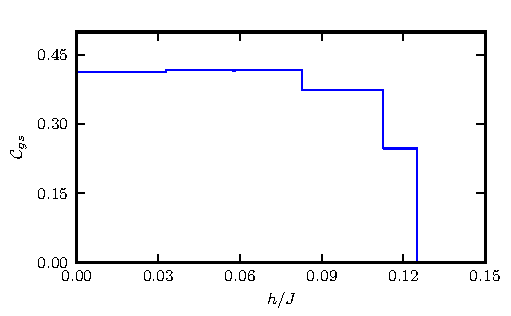
\includegraphics[width =1\textwidth]{8_chain_concurrence_varying_mag_field.pdf}
\caption{The ground-state concurrence, $\mathcal{C}_{gs}$, between two neighbouring qubits on an $N=8$ antiferromagnetic Heisenberg ring as a function of magnetic field strength in the ($z$-direction), $h$.}
\label{fig:8_chain_concurrence_varying_mag_field}
\end{center}
\end{figure}

However, when the lowest energy of a particular $M_S$ subspace is shifted so that it is higher than that of the next $M_S$, the ground-state wave function changes to one that belongs to the new $M_S$ subspace. As the form of the wave function changes so do the entanglement properties of the system. This explains, why in Fig.~\ref{fig:8_chain_concurrence_varying_mag_field} there are regions of constant entanglement. 

As the magnetic field increases, the amount of entanglement decreases as more spins are forced into alignment and the orientation of neighbouring spins becomes less correlated. Beyond a critical value of the magnetic field, $h/J = 0.125$, the concurrence drops to zero. This is the point where all spins become aligned and quantum correlations between neighbouring qubits disappears. It can be regarded as a quantum phase transition at $T=0$ due to quantum fluctuations, rather than thermal ones\cite{RudolphPrivate}.

\section{Concurrence with increasing separation}
Entanglement length\cite{Arnesen2001}, $l_E$, is another important property of many-body quantum systems that is relevant to quantum information theorists and experimentalists. It describes how quickly the entanglement between two qubits falls to zero as the separation between them is increased. 

In the Heisenberg model it is assumed that spin-spin interactions are short-range and between nearest neighbours. It is therefore difficult to find quantum correlations between spins that are not nearest neighbours. However, there is another critical value of the magnetic field, $h_{sym}$, for which an antiferromagnetic Heisenberg system is in the symmetric state
\begin{equation}
\psi_{sym} = \frac{1}{\sqrt{N}}(\ket{100\dots0} + \ket{010\dots0} + \ket{001\dots0} + \dots + \ket{000\dots1}).
\end{equation}
In this state it is evident that there is non-zero entanglement between any two qubits. This makes it possible to study how the entanglement between qubits changes as the distance between them is varied. Another benefit of this is that at this critical magnetic field the number of possible spin configurations is small and DMQMC can simulate the system very accurately.

Fig.~\ref{fig:concurrence36ChainSeparation} shows how the concurrence drops off as the distance between the two qubits increases, for an antiferromagnetic Heisenberg ring with $N=36$. Ignoring the effects near $d=0$ from the periodic boundary conditions, it can be seen that the concurrence approaches $\mathcal{C}_{gs} \propto e^{-d}$. Hence the entanglement length approaches $l_E \approx 1$. This makes sense as in the Heisenberg model it is approximated that the $J$-coupling occurs between nearest neighbours only and entanglement between non-nearest neighbours is due to non-direct interactions.
\begin{figure}[H]
\begin{center}
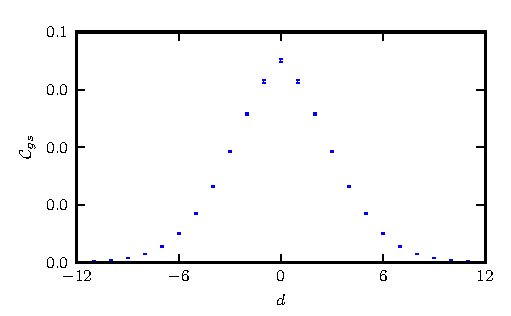
\includegraphics[width =1\textwidth]{36_chain_concurrence.pdf}\\
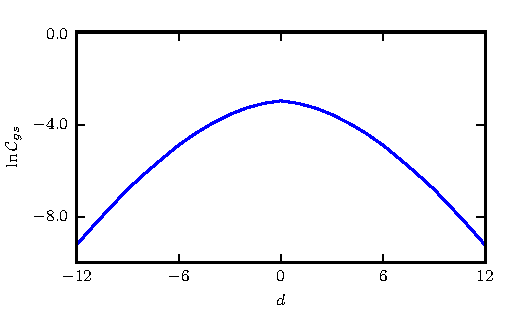
\includegraphics[width =1\textwidth]{36_log_chain_concurrence.pdf}
\caption[Ground-state concurrence with statistical errors (top) and logarithm of ground-state concurrence (bottom) for the $N=36$ antiferromagnetic Heisenberg ring, with $h/J  = 1.37$, as a function of separation between the two qubits.]{Ground-state concurrence with statistical errors (top) and logarithm of ground-state concurrence (bottom) for the $N=36$ antiferromagnetic Heisenberg ring, with $h/J  = 1.37$, as a function of separation between the two qubits. For example, $d=0$ is nearest neighbours, $d=1$ is next-nearest neighbours etc. It was difficult to obtain good statistics for $\lvert d\rvert > 10$ as the concurrence was so small. }
\label{fig:concurrence36ChainSeparation}
\end{center}
\end{figure}

\section{Summary}

In this chapter two quantum entanglement measures, the Von-Neumann entropy and the concurrence, were introduced. And the integration of these entanglement estimators into the DMQMC algorithm was discussed. The ground-state concurrence estimator was tested on one dimensional antiferromagnetic Heisenberg rings and the results were found to agree very well with the analytic values. 

Next the effects of a magnetic field on the entanglement between two nearest-neighbour qubits on an $N=8$ antiferromagnetic Heisenberg ring were studied.  It was found that there were quantum sharp transitions between different levels of entanglement due to quantum phase transitions. Finally, DMQMC was used to study how the entanglement between two qubits falls off as a function of the separation between them. It was found that there was a unit entanglement length, which agrees with the assumption in the Heisenberg model that interactions are only between nearest-neighbours.

%%% Local Variables: 
%%% mode: latex
%%% TeX-master: "../thesis"
%%% End: 

\def\baselinestretch{1}
\chapter{Conclusion}
\ifpdf
    \graphicspath{{Conclusions/ConclusionsFigs/PNG/}{Conclusions/ConclusionsFigs/PDF/}{Conclusions/ConclusionsFigs/}}
\else
    \graphicspath{{Conclusions/ConclusionsFigs/EPS/}{Conclusions/ConclusionsFigs/}}
\fi

\def\baselinestretch{1.66}

This project sought to overcome the two main restrictions of FCIQMC by stochastically sampling the many-electron thermal density matrix rather than the many-electron wave function. Although sampling the density matrix increases the computational effort because the psips now have to live, die, clone and annihilate in a space that has squared in size, it in theory allows for the calculations of any quantum mechanical observable at finite-temperatures. 

The algorithm was developed by studying an analogy between the evolution of the many-electron wave function in imaginary-time and the many-electron thermal density matrix as a function of inverse-temperature. A set of population dynamics, similar to those in FCIQMC were chosen so that they simulate a first-order finite difference approximation that relate the thermal density matrix at one inverse-temperature to the thermal density matrix at the step before. 

The DMQMC algorithm was implemented in \texttt{FORTRAN90} and built upon a current highly parallel and optimised implementation of FCIQMC. It was decided to test the implementation on some well-studied two and three dimensional antiferromagnetic bipartite Heisenberg lattices because they remove the complication of the fermion sign-problem which plagues some many-electron models. At first, it was found that the DMQMC method was far less efficient than FCI for the $4\times4$ antiferromagnetic Heisenberg lattice and actually failed for the $6\times6$ antiferromagnetic Heisenberg lattice.

It was found that the reason for this failure was that the number of psips on the trace decayed exponentially and quickly became undersampled. This was remedied by the introduction of an importance sampling method that looked to increase the sampling of rare spawning events. Under this importance sampling transformation it was found that the number of initial psips could be significantly reduced and that DMQMC could now be used to simulate larger systems for which FCI is unfeasible. 

Futhermore, larger systems such as the $4\times4\times4$ antiferromagnetic Heisenberg lattice could be simulated with a number of psips that was a only a minute fraction of the total number of elements in the thermal density matrix. As expected, DMQMC was found to be less accurate than FCIQMC for calculating ground-state properties with a similar number of psips, but it has the benefit that all of data from the simulation was useful in determining finite-temperature properties. In FCIQMC relevant data can only really be retrieved once the system is in the ground-state in the limit of large imaginary-time.

In theory it is simple to calculate the expectation value of any quantum mechanical observable in DMQMC. However, in practice it was difficult to directly sample the estimator for the heat capacity. This was due to a factor of $\beta^2$ in the estimator equation that leads to the amplification of statistical errors as $\beta$ becomes large. A solution was to calculate the derivative of the energy estimator using a cubic smoothing spline fit. However, this rather inelegant method leads to difficulties in obtaining statistical errors.

The ease of obtaining the reduced density matrix from stochastic sampling of the full thermal density matrix opened up the possibility of calculating entanglement measures and an avenue into quantum information theory. Current QMC methods do not provide access to the reduced density matrix and other methods  are non-scalable or can only simulate one dimensional systems (DMRG). So there is need for methods such as DMQMC in quantum information. Two entanglement measures, Von-Neumann entropy and concurrence, were implemented of which the ground-state concurrence estimator was tested on one dimensional antiferromagnetic Heisenberg rings for which analytic values exist. 

Some work on the DMQMC implementation is still needed. For example, the current implementation can only simulate systems within a fixed $M_S$ subspace. One needs to find a way of either simulating across all $M_S$ subspaces simultaneously or combining the results from all the different $M_S$ simulations. At this point, it would be possible to obtain the full finite-temperature picture across all $M_S$ values and it would allow for finite-temperature entanglement calculations. Additionally, it seems that the FCIQMC shift update algorithm introduces biases\footnote{There was not enough space in this report to discuss this in full.} and this problem must be solved.

In conclusion, a new QMC method has been developed. It shares some of the important features of FCIQMC, but almost fully overcomes two of FCIQMC's main restrictions at the expense of efficiency. Some more work is required, but there are signs that it could be an important QMC method for finite-temperature calculations and could be used to tackle some poorly understood aspects of quantum information theory.\\

\noindent Total words: 9997 (via TeXcount 2.3)

%%% ----------------------------------------------------------------------

% ------------------------------------------------------------------------

%%% Local Variables: 
%%% mode: latex
%%% TeX-master: "../thesis"
%%% End: 


\backmatter % book mode only
\begin{singlespace}
\begin{footnotesize}
\bibliographystyle{Classes/apsrev4-1}
%\bibliographystyle{Classes/CUEDbiblio}
%\bibliographystyle{Classes/jmb}
%\bibliographystyle{Classes/jmb} % bibliography style
\renewcommand{\bibname}{References} % changes default name Bibliography to References
\bibliography{References/FCIQMC_MSci_2011_2012,References/misc} % References file
\end{footnotesize}
\end{singlespace}

\appendix
\chapter{Appendix A: Basic electronic structure and FCIQMC}
\label{ch:appendix1}
\ifpdf
    \graphicspath{{Appendix1/Appendix1Figs/PNG/}{Chapter1/Appendix1Figs/PDF/}{Appendix1/Appendix1Figs/}}
\else
    \graphicspath{{Appendix1/Appendix1Figs/EPS/}{Appendix1/Appendix1Figs/}}
\fi
This appendix briefly reviews some of the fundamentals in electronic structure theory and projector QMC methods before moving onto a brief outline of the recent FCIQMC method.

\section*{The many-electron Schr\"{o}dinger Equation}
For a many-electron problem with $N$ electrons and $M$ nuclei the Hamiltonian, in Hartree atomic units, is
\begin{eqnarray}
\label{eq:multiHamiltonian}
 H = 
&-&\frac{1}{2}\sum_{i=1}^N \nabla_{\textbf{r}_i}^2
-\sum_{i=1}^M \frac{1}{2M_{A}} \nabla_{\textbf{r}_A}^2
-\sum_{i=1}^N \sum_{A=1}^M \frac{Z_A}{\lvert \textbf{r}_i-\textbf{d}_A\rvert}\nonumber\\
&+&\frac{1}{2}\sum_{i=1}^N \sum_{j\neq i}^N \frac{1}{\lvert \textbf{r}_i-\textbf{r}_j\rvert}
+\frac{1}{2}\sum_{A=1}^M \sum_{B\neq A}^M \frac{Z_AZ_B}{\lvert \textbf{d}_A-\textbf{d}_B\rvert},
\end{eqnarray}
where $M_A$ is the ratio of the mass of the nucleus A to the mass of an electron; $Z_A$ is the atomic number of nucleus $A$; $\textbf{r}_i$ is the position vector of the $i$th electron;  $\textbf{d}_A$ is the position vector of the $A$th nuclei. The first term in Eq.~\ref{eq:multiHamiltonian} is the kinetic energy operator of the electrons; the second term is the kinetic energy operator of the nuclei; the third term represents the electron-nuclei coulomb attraction; the fourth and fifth terms represent the electron-electron and nuclei-nuclei coulomb repulsions respectively. 

The Born-Oppenheimer approximation \cite{Born1927} assumes that the nuclei are stationary, due to the fact they are much heavier than the electrons. Hence, the second term in Eq.~\ref{eq:multiHamiltonian} can be neglected and the nuclei-nuclei repulsion term is assumed to be constant. So the time-independent many-electron Schr\"{o}dinger equation under the Born-Oppenheimer approximation becomes
\begin{equation}
\label{eq:multiElectronSE}
\left[
-\frac{1}{2}\sum_{i=1}^N \nabla_{\textbf{r}_i}^2
-\sum_{i=1}^N \sum_{A=1}^M \frac{Z_A}{\lvert \textbf{r}_i-\textbf{d}_A\rvert}
+\frac{1}{2}\sum_{i=1}^N \sum_{j\neq i}^N \frac{1}{\lvert \textbf{r}_i-\textbf{r}_j\rvert} \right]
\psi(\textbf{R}) = E\psi(\textbf{R}).
\end{equation}
The solution, $\psi(\textbf{R})$, of Eq.~\ref{eq:multiElectronSE} is the many-body wave function for $N$ electrons and is a function of the N-electron position vector $\textbf{R} = (\textbf{r}_1, \textbf{r}_2, \dotsc, \textbf{r}_N)$. Physically this can be interpreted as the probability that one electron is in region $R_1$ and that a second electron is in region $R_2$ and so on is
\begin{equation}
\label{eq:manyElectronProbability}
P(\textbf{r}_1 \in R_1 \vert \textbf{r}_2 \in R_2 \vert \dotsb \vert \textbf{r}_N \in R_N) =
\int_{R_1}d^3\textbf{r}_1\int_{R_2}d^3\textbf{r}_2\phantom{0}\dotsi \int_{R_N}d^3\textbf{r}_N\lvert\psi(\textbf{R})\rvert^2.
\end{equation}
The many-electron time-independent Schr\"{o}dinger proves extremely difficult to solve exactly because the solution is a function of $3N$ variables. Approximate solutions can be obtained by making different assumptions of varying complexity and with this complexity usually comes an increase in the computational resources required. 

\section*{Hartree-Fock method}
In quantum mechanics two electrons are fundamentally indistinguishable from one another. This and the fact that they are fermions lead to a requirement that the many-electron wave function is antisymmetric under interchange of particles;
\begin{equation}
\label{eq:antiSymmetry}
\psi(\dotsc,\textbf{x}_i,\dotsc,\textbf{x}_j,\dotsc) = - \psi(\dotsc,\textbf{x}_j,\dotsc,\textbf{x}_i,\dotsc).
\end{equation}
Where $\textbf{x}_i = \{ \textbf{r}_i, s_i\}$ represents the space and spin co-ordinates of the electron. The property in Eq.~\ref{eq:antiSymmetry} ensures that any two electrons do not have the same set of quantum numbers and hence obey the Pauli exclusion principle\cite{Foulkes2001}.

The Hartree-Fock approximation \cite{modernChemistry,bransden,James1996} is the simplest theory that correctly implements the anti-symmetric properties of the many-electron wave function. The simplest wave function with the required antisymmetry is given by the slater determinant
\begin{equation}
\label{eq:slaterDeterminant}
D(\textbf{x}_1,\textbf{x}_2,\dotsc,\textbf{x}_N) = \frac{1}{\sqrt{N!}}
\left\lvert 
\begin{array}{cccc} 
\psi_1(\textbf{x}_1) & \psi_1(\textbf{x}_2) & \dotsc & \psi_1(\textbf{x}_N) \\ 
\psi_2(\textbf{x}_1) & \psi_2(\textbf{x}_2) & \dotsc & \psi_2(\textbf{x}_N) \\ 
\vdots &\vdots &\vdots &\vdots  \\
\psi_N(\textbf{x}_1) & \psi_N(\textbf{x}_2) & \dotsc & \psi_N(\textbf{x}_N) \\ 
\end{array}
\right\rvert.
\end{equation}
The simple antisymmetric slater determinant, Eq.~\ref{eq:slaterDeterminant}, is a starting point for finding the ground state. It can be used as a variational trial function and optimised by minimising the expectation value of the hamiltonian, $ H$ with respect to each of the orbitals $\psi_i(\textbf{r})$. This leads to a set of $N$ self-consistent Hartree-Fock equations describing the single electron orbitals. The solutions to these behave as though each electron is subjected to the mean-field created by all of the other electrons.

This single determinant method includes the effects of the antisymmetry property of the many-electron wave function, Eq.~\ref{eq:antiSymmetry}, but neglects the electronic correlation arising from the electron-electron Coulomb repulsion. Correlation energies are only a small fraction of the total energy but are still important when considering binding energies \cite{Foulkes2001}. This correlation energy can be accounted for by using a linear combination of slater determinants. However, this leads to another problem as a very large number of determinants are required to accurately describe a many-electron wave function. For a full configuration-interaction calculation the number of determinants required is seen to scale exponentially with system size \cite{Foulkes2001}. This is a big problem for computational resources and other, more efficient methods must be considered to calculate ground state wave functions and energies.\footnote{One such popular method is Density Functional Theory (DFT). This has favourable $N^2-N^3$ scaling, but often fails for strongly correlated systems and non-local correlation phenomena such as van der Waals interactions
\cite{Mazzone2006}. }

\section*{Diffusion Monte Carlo and the Fermion Sign Problem}
A starting point for all ``projector'' quantum Monte Carlo methods\cite{Kent1999} is to transform the time-dependent Schr\"{o}dinger equation into imaginary time, $\tau = it$. The so-called imaginary-time Schr\"{o}dinger equation is then,
\begin{equation}
\label{eq:imaginaryTime}
\frac{\partial \psi}{\partial \tau} = - H\psi,
\end{equation}
where $\psi$ is the time-dependent many-electron wave function. A formal solution to the imaginary-time Schr\"{o}dinger equation can be written,
\begin{equation}
\label{eq:imaginaryTimeSolution}
\psi(\tau_1 + \delta \tau) = e^{-H\delta\tau}\psi(\tau_1).
\end{equation}
The state $\psi$ evolves in imaginary time over a duration of $\delta\tau$. If the initial state, $\psi(\tau_1)$, is expanded as a linear combination of ordered energy eigenstates, $\phi_i$, with $\epsilon_0 < \epsilon_1 < \dotsb < \epsilon_{\infty}$, then
\begin{equation}
\label{eq:imaginaryTimeSolutionExpansion}
\psi(\delta \tau) = \sum_{i=0}^{\infty}c_i e^{-\epsilon_i \delta\tau}\phi_i.
\end{equation}
From this it is then obvious that any initial state, $\psi$, that is not orthogonal to the ground-state, $\phi_0$, will evolve to the ground state in the long-time limit,
\begin{equation}
\label{eq:longTimeLimit}
\lim_{\tau \to \infty} \psi = c_0 e^{-\epsilon_0 \delta\tau}\phi_0.
\end{equation}
The ground-state is therefore projected out. The aim of all Monte Carlo projector methods, such as Diffusion Monte Carlo (DMC)\cite{Sorella1989}, is to perform a stochastic long-time integration of Eq.~\ref{eq:imaginaryTime} in order to retrieve the ground-state. 

If the hamiltonian in Eq.~\ref{eq:imaginaryTime} is expanded in terms of the kinetic energy and potential terms\footnote{An adjustable constant energy offset, $E_T$, is introduced in order to keep Eq.~\ref{eq:longTimeLimit} finite.}, the imaginary-time Schr\"{o}dinger equation takes on a form that is analogous to the diffusion equation:
\begin{equation}
-\frac{\partial}{\partial\tau}\psi(\textbf{R},\tau)= \left[-\frac{1}{2}\sum_{i=1}^N \nabla_{\textbf{r}_i}^2 + V(\textbf{R})-E_T\right]\psi(\textbf{R},\tau).
\end{equation}
Here, $\psi(\textbf{R},\tau)$ may be interpreted as the density of diffusing particles and $(V(\textbf{R})-E_T)$ as a rate term describing a potential-dependent change in the particle density. In the Monte Carlo literature these particles are known as ``walkers''.

\begin{figure}[h!]
\begin{center}
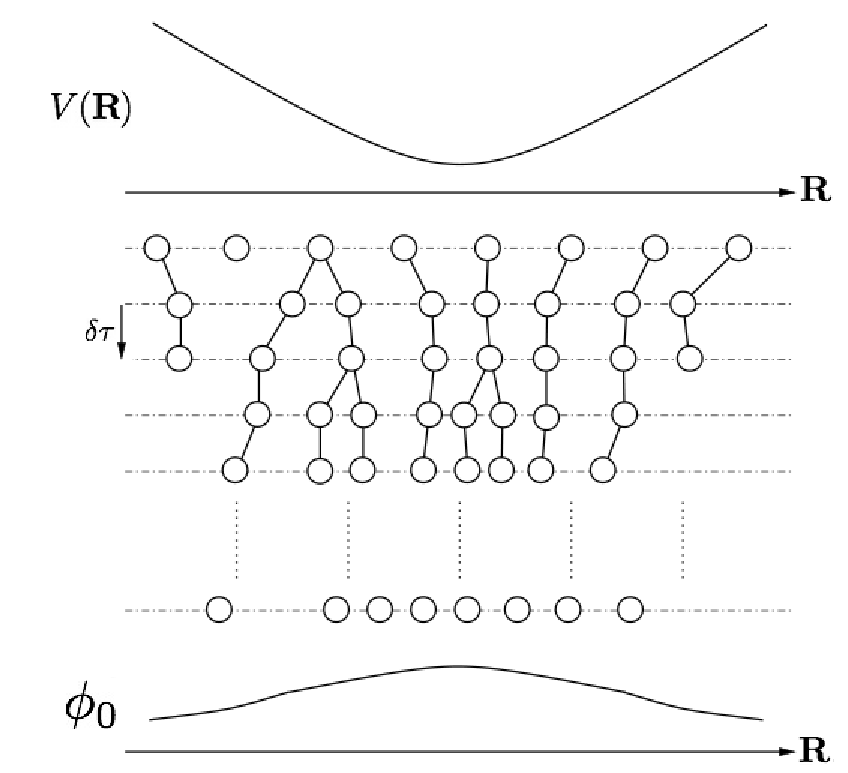
\includegraphics[width =0.49\textwidth]{DMC.pdf}
\caption[Illustration of the diffusion of walkers in DMC]{The diffusion of walkers through \textbf{R}-space. An initially even distribution of walkers is propagated through imaginary time, $\tau$. Under the influence of the potential $V(\textbf{R})$,  the distribution eventually evolves into what is representative of the ground state many-electron wave function $\psi(\textbf{R})$.}
\label{fig:DMC}
\end{center}
\end{figure}
%\begin{wrapfigure}{r}{0.3\textwidth}
%\begin{center}
%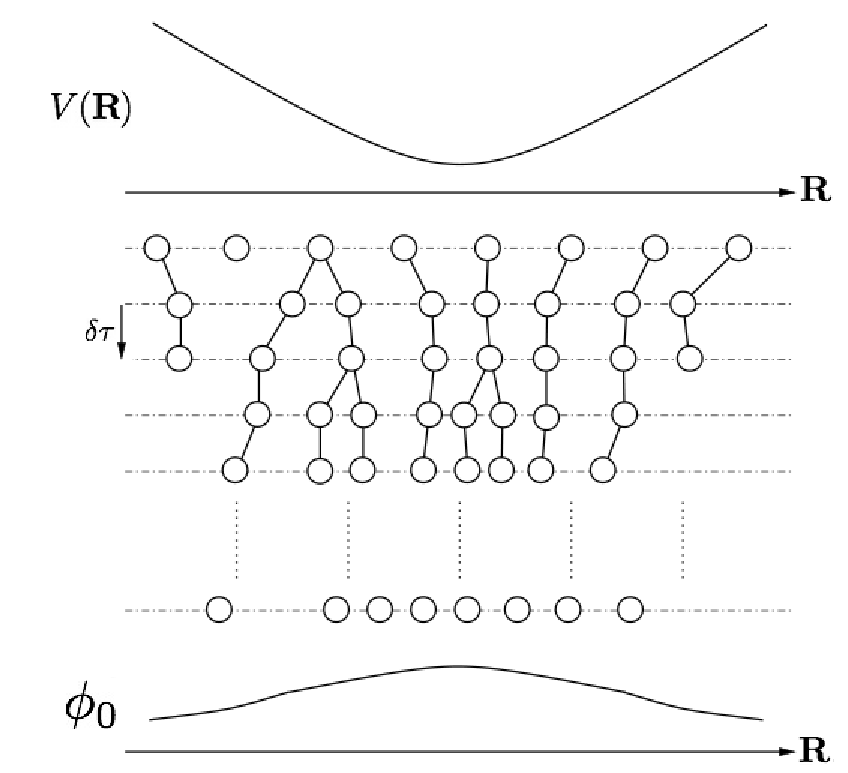
\includegraphics[width =0.3\textwidth]{DMC.pdf}
%\caption{The diffusion of walkers through \textbf{R}-space. An initial even distribution of walkers is propogated through imaginary time, $\tau$. Under the influence of the potential $V(\textbf{R})$,  The distribution eventually evolves into what is representative of the ground state many-electron wave function $\phi_0(\textbf{R})$.}
%\label{fig:Setup}
%\end{center}
%\end{wrapfigure}

It is well known that the only major obstacle preventing the exact solution of the many-electron  Schr\"{o}dinger equation via stochastic methods, such as DMC, is the fermion sign problem. This problem arises from the antisymmetry of many-electron wave functions, Eq.~\ref{eq:antiSymmetry}. As the  Schr\"{o}dinger equation becomes a diffusion equation in imaginary time, Eq.~\ref{eq:imaginaryTime}, its lowest energy solution is generally symmetric and nodeless, which directly disagrees with fermion antisymmetry. Stochastic propagation leads directly to this undesired solution in a process known as the ``boson catastrophe''\cite{Booth2009}.

One way of trying to prevent the boson catastrophe  is the fixed-node approximation\cite{Foulkes2001,BajdichMichalandMitas2009}. In this, a trial function is used to predict positive and negative regions of the wave function, thus defining a nodal surface. If a walker attempts to cross a node then it is rejected, hence constraining the propagation to disjoint areas of propagation. This procedure would be exact if the applied nodal boundaries coincided with the exact nodal hypersurface of the ground-state electronic wave function~\cite{Booth2009}. It has in fact proven very difficult to determine accurate fixed-node surfaces for large systems. 

\section*{Full Configuration-Interaction Quantum Monte Carlo}
In 2009 Booth, Alavi and Thom \cite{Booth2009} introduced a new quantum Monte Carlo method for the simulation of correlated many-electron systems in full configuration-interaction spaces. The new method is designed to simulate the many-electron imaginary-time Schr\"{o}dinger using a set of walkers that inhabit Slater determinant space, $\{D_i \}$, and evolve under the guidance of a simple set of rules; spawning, cloning, death and annihilation. The inventors of FCIQMC note three key elements of the algorithm;
\begin{enumerate}
\item As with DMC a long-time integration of the imaginary-time Schr\"{o}dinger equation is performed, however it is achieved in a space of Slater determinants
\item In a similar way to DMC the instantaneous wave function is represented by walkers instead of amplitude coefficients, allowing the description of the FCI wave function stochastically, without storing all amplitudes simultaneously
\item Walkers carry a positive or negative sign which allows for annihilation, where two walkers of opposite sign are destroyed if they coincide on the same determinant
\end{enumerate}

In order to satisfy these three key elements a long-time integration must be performed on an analogue of Eq.~\ref{eq:imaginaryTime} that is expressed in a Slater determinant basis. A set of coupled first-order differential equations for the FCI coefficients are derived\cite{Booth2009}:
\begin{equation}
\label{eq:schrodingerSlaterSpace}
-\frac{dC_i}{d\tau} = (K_{ii}-S)C_i + \sum_{j\neq i}K_{ij}C_j,
\end{equation}
where
\begin{equation}
\label{eq:KMatrixElements}
K_{ij} \equiv \Bra{D_i} K \Ket{D_j} = \Bra{D_i} H\Ket{D_j}-E_{HF}\delta_{ij},
\end{equation}
where $S$ is an adjustable energy offset\footnote{Similar to in DMC this energy offset is introduced to keep the population under control}, $C_j$ is the coefficient of the $j$th determinant in the Slater determinant expansion of the wave function (CI coefficients) and $E_{HF}$ is the Hartree-Fock energy. 

The population dynamics algorithm \cite{Booth2009,Booth2010,Booth2011} simulates the set of differential equations, Eq.~\ref{eq:schrodingerSlaterSpace}. The algorithm consists of three steps, which are performed at each time step of length $\delta\tau$:
\begin{enumerate}
\item \underline{Spawning:}  Each walker located on $D_i$ attempts to spawn another walker on a connected determinant $D_j$ with probability 
\begin{equation}
P_s(D_j\vert D_i) = \frac{\delta \tau \lvert K_{ij} \rvert}{P_{gen}(D_j\vert D_i)},
\end{equation}
where $P_{gen}(D_j\vert D_i)$ is the calculated probability of generating $D_j$\footnote{Booth \textit{et al.}\cite{Booth2009} describe how to calculate $P_{gen}$}. The sign of the spawned walker is the same as the parent if $K_{ij}<0$ and is opposite otherwise.
\item \underline{Diagonal death/cloning:} For each parent (pre-existing walker) compute
\begin{equation}
p_d(D_i) = \delta\tau(K_{ii}-S).
\end{equation}
If $p_d > 0$ the walker dies (immediately removed from simulation) with probability $p_d$ otherwise it is cloned with probability $\lvert p_d \rvert$.
\item \underline{Annihilation:} run over all remaining walkers and annihilate all opposite-sign pairs that occupy the same point in antisymmetric Slater determinant space.
\end{enumerate}
%\begin{figure}[h!]
%\begin{center}
%\includegraphics[width =0.49\textwidth]{FCIQMC.eps}
%\caption{Illustration of the spawning, cloning, death and anhilation processes as a walker %population, consisting of $+$ and $-$ signs, evolves in a Slater determinant space in imaginary %time, $\tau$. Eventually the walker population reaches a critical number and the walker growth %exhibits a characteristic plateau at which point the correlation energy can be extracted.}
%\label{fig:FCIQMC}
%\end{center}
%\end{figure}
Such an algorithm converges on the exact fermonic ground-state of the Hamiltonian in the Slater determinant basis~\cite{Booth2009}. So in this way, it prevents convergence to a bosonic solution, which is a major problem in other QMC methods. Moreover, FCIQMC simulations do not require any \emph{a priori} information and hence removes the hassle of trying to calculate a nodal structure as is inherent in DMC. 

% ------------------------------------------------------------------------

%%% Local Variables: 
%%% mode: latex
%%% TeX-master: "../thesis"
%%% End: 

\chapter{Appendix B: $C_h$ spline derivative estimator}
This appendix includes more detail on the calculation of the heat capacity in a uniform magnetic field using the derivative of the DMQMC finite-temperature energy estimator.

\section*{Smoothing spline fit}
In Sec.~\ref{sec:heatCapacity} it was found that the heat capacity in a uniform magnetic field could be expressed as
\begin{equation}
C_{h} = -\beta^2\frac{d\langle H\rangle}{d\beta}.
\end{equation}

The problem here is that the $\langle H\rangle$ data contains statistical noise and it thus proves difficult to obtain an accurate approximation of the gradient function. However, it is possible to fit a smooth curve to the data using a smoothing spline\cite{Reinsch}. A spline is essentially a piece-wise polynomial. The data is split into regions and each region is approximated by a polynomial, usually a cubic.

For a sequence of measurements $M_i$ that can be modelled as $M_i =F(x_i)$, where $\{ x_i \lvert x_1 < x_2 < \dots < x_N, x_i \in \mathcal{Z} \}$ and $F$ is some function, the smoothing spline estimate $\bar{F}$ of $F$ is defined as the function that minimises 
\begin{equation}
\sum^n_{i=1} (M_i - \bar{F}(x_i))^2 + \eta \int_{x_1}^{x_N} \bar{F}''(x)^2 dx.
\end{equation}
Here $\eta \geq 0$ is the smoothing parameter which controls the smoothing characteristics $\bar{F}$. For $\eta \to 0$ $\bar{F}$ becomes an interpolating spline and for $\eta \to \infty$ $\bar{F}$ converges to a linear least squares estimate. 

\texttt{Python} has a smoothing spline implementation, \texttt{splev}, in the \texttt{scipy.interpolate} sub-package. In this the smoothing parameter is chosen so that it is between $N-\sqrt{2N} < \eta < N+\sqrt{2N}$ and the best fit of the data can be found by trial and error. The \texttt{splev} function can also return derivatives of $\bar{F}$, which proved useful for calculating the $C_h$.

So during this investigation the DMQMC spline derivative estimate of $C_h$ was determined in a post-processing step. This step was inelegant as it relied on some trial and error and it was difficult to obtain errors.





%%% Local Variables: 
%%% mode: latex
%%% TeX-master: "../thesis"
%%% End: 

\chapter{Appendix C: Code}

This appendix presents some of the main components of the DMQMC implementation in \texttt{FORTRAN 90} that were developed during this project. The \texttt{dmqmc} module in Code 1 contains the main outline of the algorithm as presented in Sec.~\ref{sec:implementation}. \texttt{dmqmc\_procedures.f90} and \texttt{dmqmc\_estimators.f90} in Code 2 and Code 3 contain some important general procedures and the implementation of the estimators respectively.

\lstset{
columns=fullflexible,
basicstyle=\ssmall\ttfamily,
language=Fortran,
numbers=left,
numberstyle=\tiny,
frame=tb,
columns=fullflexible,
breaklines=true,        % sets automatic line breaking
breakatwhitespace=false,    % sets if automatic breaks should only happen at whitespace
showspaces=false,               % show spaces adding particular underscores
showstringspaces=false,         % underline spaces within strings
showtabs=false,                 % show tabs within strings adding particular underscores
tabsize=2,          % sets default tabsize to 2 spaces
keywordstyle=\color{blue},          % keyword style
commentstyle=\color{dkgreen},       % comment style
stringstyle=\color{mauve},         % string literal style
}

\lstinputlisting[caption=dmqmc.f90, label = dmqmc]{dmqmc.f90}
\newpage
\lstinputlisting[caption = dmqmc\_procedures.f90, label = procs]{dmqmc_procedures.F90}
\newpage
\lstinputlisting[caption= dmqmc\_estimators.f90, label = ests]{dmqmc_estimators.F90}

%%% Local Variables: 
%%% mode: latex
%%% TeX-master: "../thesis"
%%% End: 


\end{document}
